\chapter{Protei\textbf{n} Folding}
{
\say{\textit{la forma è l'immagine plastica	della funzione}}\footnote{\fullcite{ruffini1925fisiogenia}}\\

La correlazione tra forma e funzione si rivela fondamentale nel caso delle proteine. Un canale ionico neuronale permette il passaggio di ioni grazie alla sua forma a canale; una \textit{ferritina} cattura e immagazzina gli ioni ferro grazie alla sua forma a sfera cava. 

\begin{figure}[htp]
	\centering
	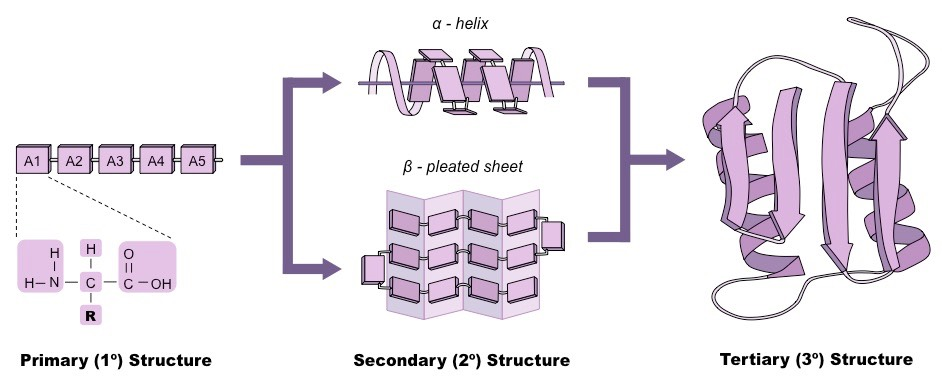
\includegraphics[scale=0.5]{images/protein-folding_med.jpeg}
	\caption{Protein folding: dagli amminoacidi alla struttura tridimensionale. Fonte: \cite{proteinStrucBioNinja}}
	\label{fig:protein-folding-bioninja}
\end{figure}

\par Il ripiegamento delle proteine (\textit{protein folding}) è il processo di ripiegamento molecolare attraverso il quale a partire dalla sequenza lineare amminoacidica le proteine ottengono la loro struttura tridimensionale, chiamata forma \textit{nativa}, che permette loro di svolgere la relativa funzione biologica\footnote{Per una trattazione superficiale della mancanza di generalità di questo paradigma si veda la sezione \ref{sfide-dogma}. Per una scrittura e lettura più agevole della presente tesi si è preferito accettare la visione del paradigma.}. 

\par Il ripiegamento nella forma tridimensionale avviene spontaneamente sia durante la sintesi proteica nei ribosomi sia al termine di questa. Una specifica proteina si ripiegherà nello stesso modo e avrà la stessa struttura finale\footnote{Ciò non è vero nel 100\% dei casi, alcune proteine possono avere più di una conformazione stabile per adempiere funzioni diverse (vedi la sezione \ref{sec:fold-switching-proteins}) e alcune proteine possono andare incontro a misfolding (vedi la sezione \ref{sec:assisted-folding}).}.

\par La prima teoria del ripiegamento proteico è stata proposta negli anni venti del XX secolo da Hsien Wu\supercite{wu1931studies}, in relazione al processo di denaturazione (vedi sezione \ref{sec:denaturazione}). È però Anfinsen, premio Nobel per la chimica, negli anni '60 a compiere un fondamentale passo nella comprensione del processo del ripiegamento proteico\supercite{anfinsen1972formation}. 

}
\section{Postulato di Anfinsen}
{
Il postulato di Anfinsen (conosciuto anche come \textit{dogma} o \textit{ipotesi termodinamica} di Anfinsen) afferma che la struttura nativa di una proteina è determinata dalla sua sequenza di amminoacidi, sotto condizioni native. In altri termini: la struttura nativa, in ambiente fisiologico standard, corrisponde a quella struttura unica, stabile e cineticamente accessibile avente \textit{minima energia libera}. 

\begin{figure}[h]
	\centering
	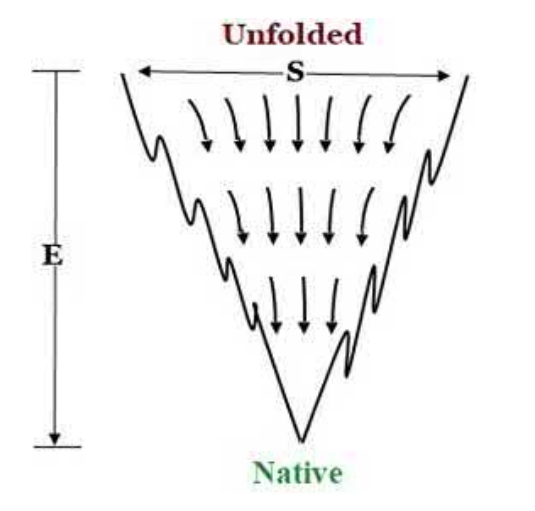
\includegraphics[scale=0.3]{images/funnel-folding.png}
	\caption{Un profilo energetico idealizzato dell'energia libera a forma di imbuto. E=energia, S=entropia. Fonte: \cite{pal2019fundamentals}}
	\label{fig:funnel}
\end{figure}

Vi sono quindi 3 condizioni:

\begin{enumerate}
	\item \textit{unicità}, la sequenza non deve possedere altre configurazioni dotate di energia libera comparabile
	\item \textit{stabilità}, piccoli cambiamenti nell'ambiente circostante non possono produrre cambiamenti nella configurazione a energia minima. Ciò può essere descritto come una superficie parabolica di energia libera con lo stato nativo corrispondente al punto di minimo (visivamente simile ad un imbuto, vedi fig. \ref{fig:funnel}); la superficie di energia libera nelle vicinanze dello stato nativo deve essere abbastanza ripida ed elevata
	\item \textit{accessibilità cinetica}, il percorso nella superficie di energia libera dallo stato \textit{unfolded} a \textit{folded} deve essere ragionevolmente piano
\end{enumerate}


\subsubsection{Esperimento di Anfinsen}
{
L'esperimento, compiuto nel 1957\supercite{anfinsen1961kinetics}, consisteva nella denaturazione e rinaturazione della ribonucleasi A, dimostrando che il secondo processo era possibile senza agenti ausiliari. L'enzima in questione è formato da 124 amminoacidi, tra cui 8 cisteine che formano 4 ponti disolfuro ($-CH_{2}-\textbf{S-S}-CH_{2}-$, vedi sez. \ref{sec:legami-chimici}). È stato usato un agente riducente per scindere questi ponti e l'urea per denaturare la proteina: questa non mostrava più alcuna attività enzimatica. A questo punto se l'urea era rimossa prima, seguita dall'aggiunta di un agente ossidante per consentire ai ponti disolfuro di riformarsi, la ribonucleasi A riacquistava spontaneamente la sua struttura terziaria e il prodotto ottenuto risultava praticamente indistinguibile dalla proteina nativa di partenza, riottenendo piena attività biologica. 

\begin{figure}[h]
	\centering
	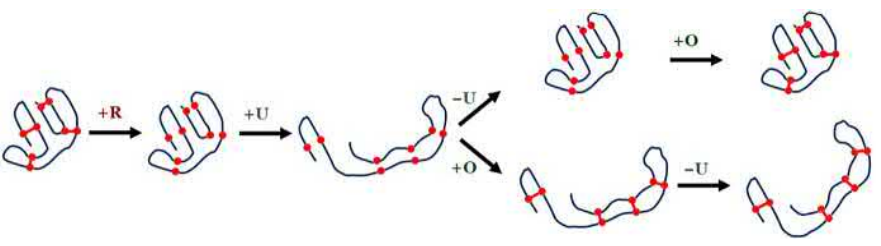
\includegraphics[scale=0.6]{images/anfinsen-experiment.png}
	\caption{Rappresentazione schematica dell'esperimento di Anfinsen. R=reducing agent, U=Urea, O=oxidizing agent, punti rossi=cisteina, linee rosse=ponti disolfuro. Fonte: \cite{pal2019fundamentals}}
	\label{fig:anfinsen-exp}
\end{figure}

I ponti disolfuro si riformano nella stessa posizione della proteina nativa nonostante ci siano 105 modi possibili per ricombinarli. Se invece veniva prima aggiunto l'agente ossidante e poi tolta l'urea il prodotto ottenuto era un miscuglio di molte delle possibili 105 configurazioni, raggiungendo solamente l'1\% dell'attività enzimatica.

\begin{figure}[!htb]
	\minipage{0.45\textwidth}
	\centering
	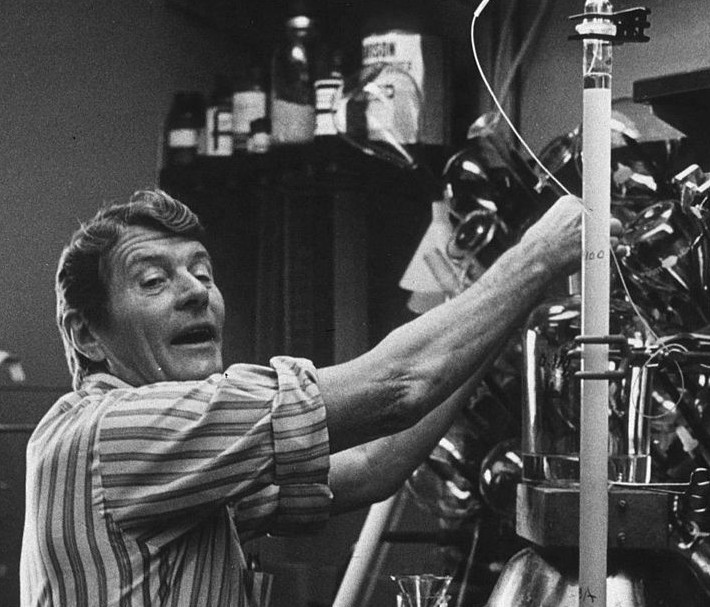
\includegraphics[scale=0.25]{images/anfinsen.jpg}
	\caption{C.B. Anfinsen nel suo laboratorio. Fonte: \cite{anfinsenNIH}}
	\label{fig:anfinsen}
	\endminipage\hfill
	\minipage{0.5\textwidth}
	\centering
	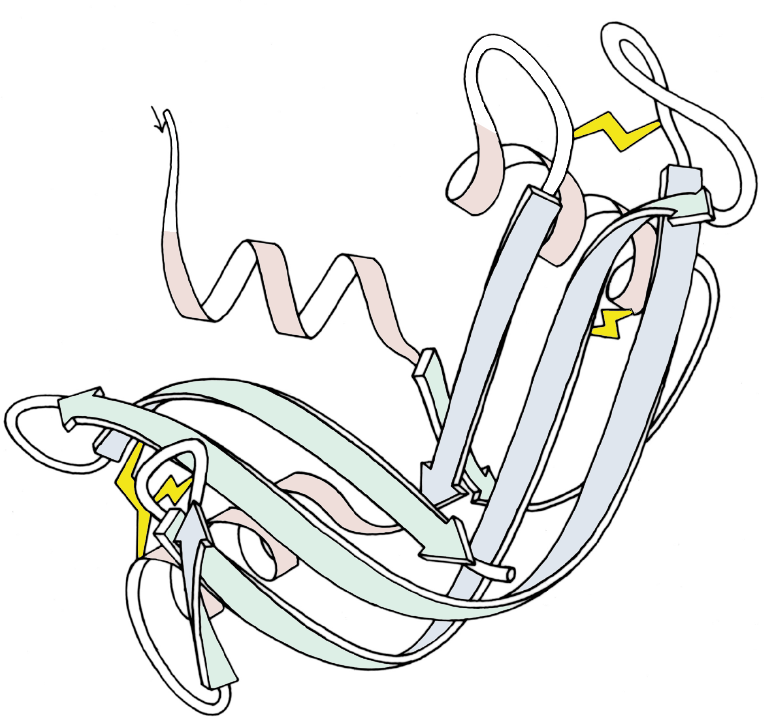
\includegraphics[scale=0.2]{images/RibonucleaseA_SS_paleRib.png}
	\caption{Ribonucleasi A, rappresentazione a nastro. In giallo i ponti disolfuro, rosa le $\alpha$-eliche, verde e azzurro i $\beta$-foglietti. Fonte \cite{ribonucleasi-file}}
	\label{fig:ribonucleasi}
	\endminipage\hfill
\end{figure}

Dai lavori di Anfinsen è possibile trarre due ulteriori importanti conclusioni\supercite{dill2008protein}:
\begin{itemize}
	\item ha dato via alla grande avventura della ricerca nel campo del protein folding \textit{in vitro}\footnote{La locuzione latina \textit{in vivo} significa \textit{nel vivente}. Se il fenomeno biologico viene riprodotto in una provetta si dice \textit{in vitro} mentre se lo si riproduce tramite una simulazione computazionale si dice \textit{in silico}.} piuttosto che all'interno di cellule. La struttura nativa non dipendeva quindi dal fatto che la proteina fosse sintetizzata biologicamente con l'aiuto di ribosomi (ed eventualmente chaperoni molecolari) o che si ripiegasse nuovamente come molecola isolata all'interno di una provetta
	\item l'evoluzione può agire in modo da cambiare la sequenza amminoacidica ma l'equilibrio del ripiegamento e la cinetica di una data sequenza sono materia della fisica chimica.
\end{itemize}}

}

\subsection{Denaturazione} \label{sec:denaturazione}
{
La denaturazione delle proteine è il fenomeno relativo all'alterazione della struttura nativa dovuto a variazioni di temperatura, pH o contatto con determinate sostanze chimiche. La denaturazione è un processo che porta alla perdita di ordine e quindi ad un aumento di entropia. La struttura primaria rimane invariata, data la stabilità dei legami peptidici. A causa della denaturazione le proteine perdono la loro funzione biologica e possono esporre e rendere reattivi alcuni gruppi funzionali che possono causare l'aggregazione di più proteine. Può avvenire che una volta rimosso l’agente denaturante la proteina ritorni allo stato di partenza (\textit{rinaturazione}) ma spesso il processo è irreversibile.

\begin{figure}[h]
	\centering
	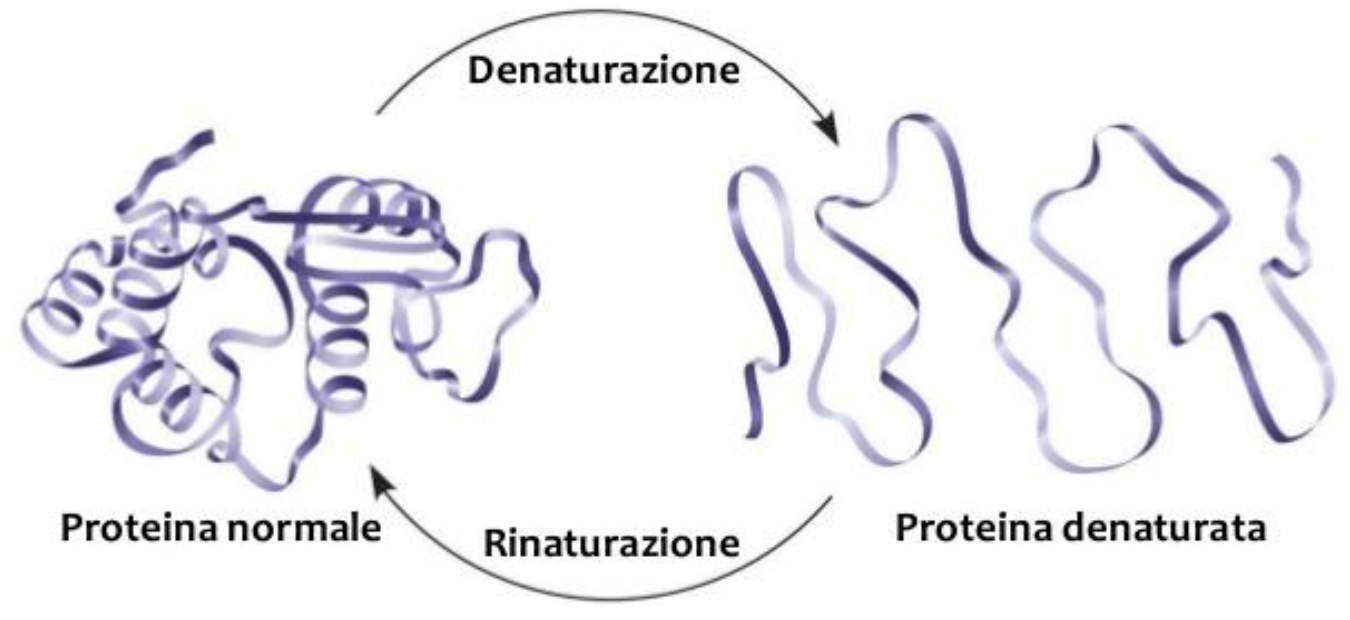
\includegraphics[scale=0.3]{images/denaturazione-rina.png}
	\caption{Denaturazione e rinaturazione. Fonte: \cite{campbell}}
	\label{fig:denaturazione}
\end{figure}

\par La proprietà di certe sostanze chimiche (es. urea) di denaturare una molecola proteica si deve alla loro capacità di legare transientemente, attraverso legami deboli, come ad esempio legami idrogeno, i residui amminoacidici costituenti la proteina. Questi legami vengono termodinamicamente preferiti a quelli intramolecolari o intermolecolari con l'acqua. Ciò comporta l'impossibilità per la proteina di mantenere la propria struttura tridimensionale e quindi questa si denatura. 

\par Applicazioni nella vita quotidiana di questo fenomeno sono la cottura dei cibi (basti pensare all'albumina nell'uovo) e la permanente ai capelli (denaturazione dell' $\alpha$-cheratina, rompendo e riformando ponti disolfuro). 
}

\section{Struttura delle proteine}
{
Da un punto di vista chimico le proteine sono di gran lunga, tra quelle conosciute, le molecole strutturalmente più complesse e sofisticate funzionalmente. È possibile studiare la loro struttura individuando successivi livelli di organizzazione:

\begin{figure}[!htp]
	\centering
	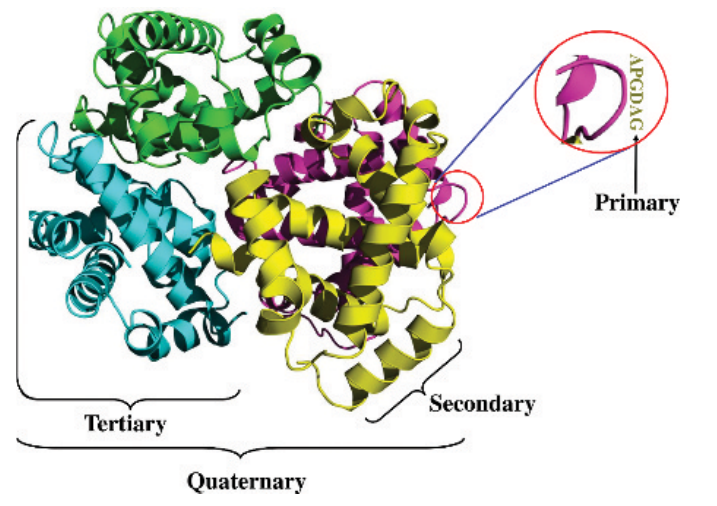
\includegraphics[scale=0.5]{images/strutture-proteina.png}
	\caption{Livelli strutturali di una proteina. Fonte: \cite{kessel_ben-tal_2018}}
	\label{fig:strutture-proteine}
\end{figure}

\begin{itemize}
	\item \textit{struttura primaria}: la sequenza ordinata degli amminoacidi
	\item \textit{struttura secondaria}: regioni ripetitive locali stabilizzate da legami idrogeno tra atomi della backbone ($\alpha$-eliche e $\beta$-foglietti)
	\item \textit{struttura supersecondaria}: combinazione di strutture secondarie e connessioni (motivi, domini, loop, giri ecc.)
	\item \textit{struttura terziaria}: forma tridimensionale di una singola catena polipeptidica, risultante dalle interazioni dei residui
	\item \textit{struttura quaternaria}: forma finale di proteine "assemblate" da 2 o più catene polipeptidiche già ripiegate
\end{itemize}

Prima di passare ad analizzare ogni livello della struttura delle proteine è utile un veloce sguardo ai legami chimici e  alle interazioni molecolari.

\subsection{Legami e interazioni molecolari} \label{sec:legami-chimici}
{
	La chimica della vita è di un tipo speciale: è una chimica organica formata da composti carboniosi, in un ambiente acquoso, con temperature "terrestri" e complicata, basata su grandi polimeri. Gli atomi possono risultare incompleti, e grazie a questo formare legami per completarsi. Elementi puri e pienamente completi non trovano spazio nella chimica della vita. Nei viventi solo gli elettroni si spostano\footnote{Protoni e neutroni si separano solo in condizione estreme: nei reattori nucleari, nel sole, per decadimento radioattivo.} per ricercare stabilità, ovvero per permettere agli atomi di completare il loro guscio orbitale più esterno. Ogni atomo può avere tanti \textit{legami} quanti elettroni gli mancano per completare il suo guscio più esterno.	Le \textit{interazioni molecolari }sono forze attrattive o repulsive tra molecole e tra atomi
	non legati. La \textit{forza di legame} è la misura dell'energia necessaria per romperlo (in kJ/mol o kcal/mol). Si elencano ora i principali legami inerenti al ripiegamento delle proteine:
		
\begin{itemize}
	\item \textit{legame covalente}: prevede la compartecipazione di 2 elettroni di valenza fra più atomi ed è il tipo di legame più forte. Due o più atomi tenuti insieme da legami covalenti formano una molecola. C'è una specifica distanza di legame fra i nuclei degli atomi bilanciata tra forze attrattive e repulsive: se sono troppo vicini c'è repulsione mentre se sono troppo lontani non c'è attrazione.
		\begin{itemize}
			\item \textit{elettronegatività}: spesso gli elettroni in un legame sono condivisi iniquamente. Questo dipende dall'elettronegatività degli atomi, ad esempio l'ossigeno ha elettronegatività 3.4 mentre l'idrogeno 2.1. Quando la differenza di elettronegatività è compresa tra 0.5 e 1.9 la nube elettronica di legame risulta deformata verso l'atomo più elettronegativo, su cui si origina una carica parziale negativa (indicata con $\delta^{-}$) mentre l'altro atomo acquisisce una carica parziale positiva di uguale valore assoluto. La molecola, divenuta \textit{polare}, si può immaginare ora come un \textit{dipolo }elettrico.

			\item \textit{ponti disolfuro}: i legami (o ponti) disolfuro sono legami covalenti tra due atomi di zolfo con energia di legame di 60kcal/mol. Si formano dall'accoppiamento di due gruppi tiolici (-SH). Essendo legami molto forti costituiscono un elemento architetturale fondamentale nella struttura delle proteine. La cisteina presenta un gruppo -SH nella catena laterale e può quindi formare ponti disolfuro.
		\end{itemize}
		
		\begin{figure}[!htp]
			\centering
			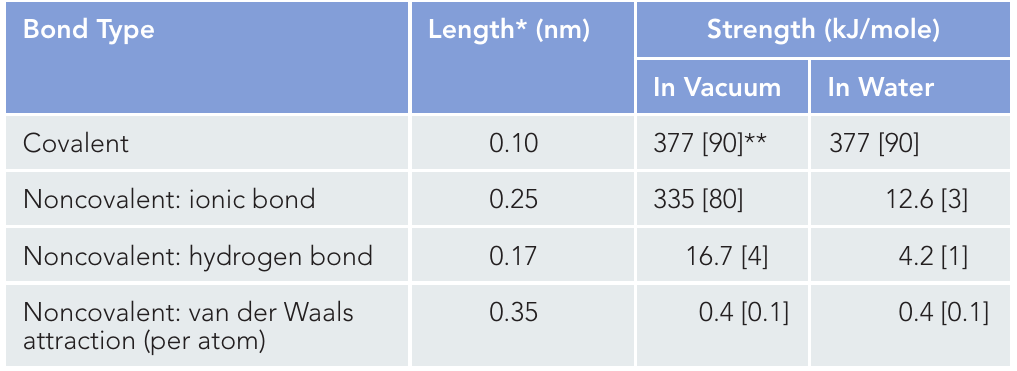
\includegraphics[scale=0.5]{images/forza-legami.png}
			\caption{Distanza di legame approssimate e forza dei legami chimici. I valori della forza sono riportati in kJ/mol e in [kcal/mol]. Da notare la diminuzione di forza nel legame ionico se in ambiente acquoso. Fonte: \cite{alberts2018essential}}
			\label{fig:forza-legami}
		\end{figure}
	
	\item \textit{legami non covalenti (interazioni molecolari)}
		\begin{itemize}
			
			\item \textit{attrazioni elettrostatiche}: le forze d’attrazione agiscono fra gruppi completamente carichi (legame ionico) e fra i gruppi parzialmente carichi
			delle molecole polari. Decresce con la distanza. Molto deboli in acqua.
			
			\begin{itemize}
				\item \textit{legame ionico}: l'atomo più elettronegativo strappa completamente un elettrone al suo compagno, si formano due ioni (uno positivo, \textit{catione} e uno negativo \textit{anione}). Si ha quando la differenza di elettronegatività tra i due atomi è maggiore di 1.9. 
			\end{itemize}		
			\item \textit{legame idrogeno}: è una forza dipolo-dipolo che si origina tra molecole contenenti un atomo di idrogeno unito covalentemente a ossigeno, fluoro o azoto. Un atomo di idrogeno elettropositivo è parzialmente condiviso da due atomi elettro-negativi; ad es. nell'acqua gli atomi di idrogeno (parzialmente positivi) si trovano fra due atomi di ossigeno (parzialmente negativi). L'idrogeno, legato a uno dei due atomi di ossigeno, permette all'altro di avvicinarsi e di stabilizzare le molecole. Sono legami deboli singolarmente (1/20 della forza di un legame covalente) ma quando se ne formano simultaneamente molti sono abbastanza forti da fornire un legame stretto  (l'acqua bollirebbe a -120°C senza legami idrogeno).
			
			\begin{figure}[!htp]
				\centering
				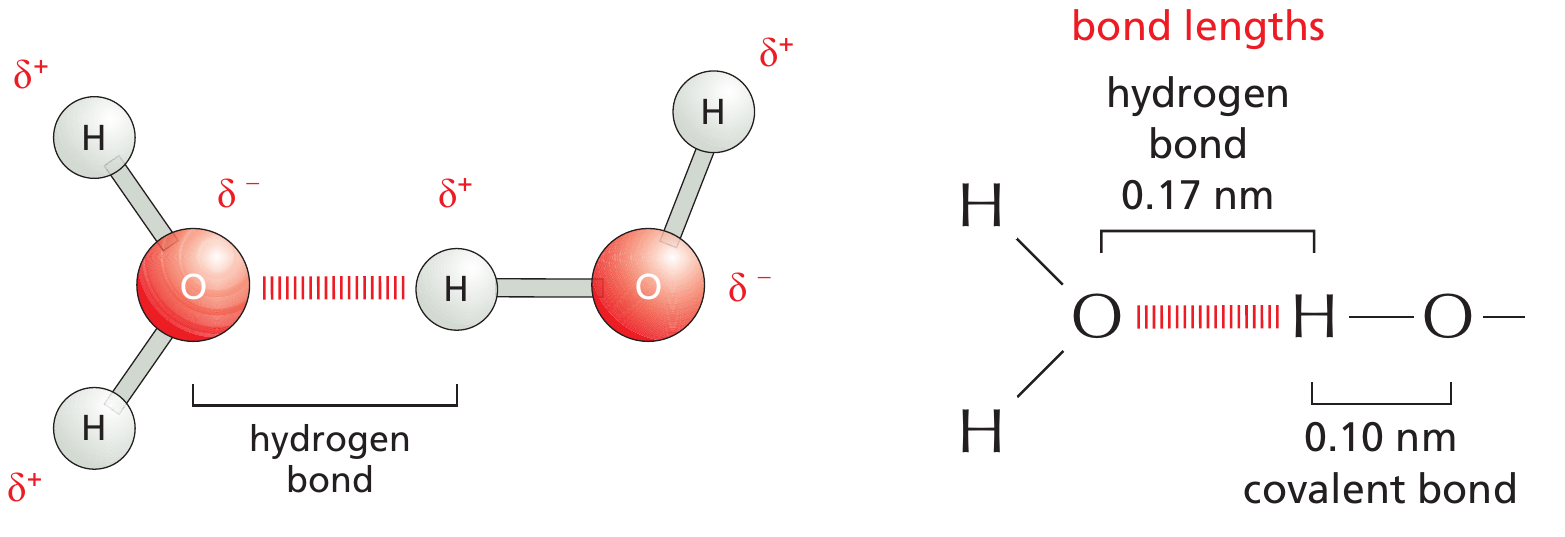
\includegraphics[scale=0.25]{images/legame-idrogeno.png}
				\caption{Legame idrogeno tra due molecole d'acqua. Fonte: \cite{alberts2018essential}}
				\label{fig:legame-idrogeno}
			\end{figure}
			
			\item \textit{interazioni di van der Waals}: nelle molecole apolari gli elettroni si possono accumulare in modo asimmetrico, formando regioni momentaneamente polari che permettono così una temporanea stabilizzazione fra molecole a breve distanza. Due atomi saranno attratti l’uno dall’altro fino a che la distanza fra i loro nuclei è			approssimativamente uguale alla somma dei loro raggi di van der Waals (ad es. per il carbonio il raggio è di 0.2$nm$)
		\end{itemize}
	\item \textit{forze idrofobiche}: l’acqua forza insieme i gruppi idrofobici; l’apparente attrazione è in realtà causata da una repulsione dall’acqua, che difende il suo reticolo tenuto insieme da legami idrogeno.
			\begin{figure}[!htp]
				\centering
				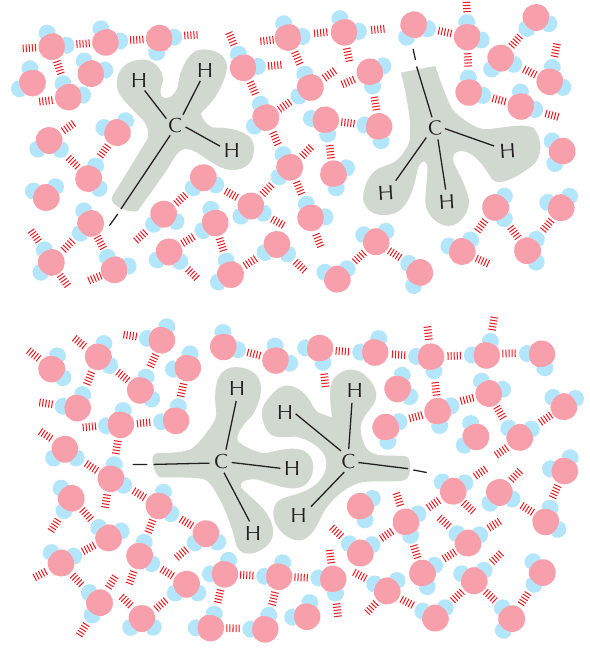
\includegraphics[scale=0.3]{images/forze-idrofobiche.png}
				\caption{Forze idrofobiche. Fonte: \cite{alberts2018essential}}
				\label{fig:effetto-idrofobico}
			\end{figure}
		
	Le sostanze \textit{idrofile} si dissolvono rapidamente nell'acqua poiché le loro molecole formano legami idrogeno con le circostanti molecole d'acqua (nel caso di sostanze polari) o perché queste sono attratte dalle cariche degli ioni (nel caso di sostanze ioniche, es. cloruro di sodio, con ioni $Na^{+}$ e $Cl^{-}$). Le sostanze \textit{idrofobiche} contengono perlopiù legami non polari e sono solitamente insolubili in acqua. Le molecole d'acqua in questo caso non sono attratte ma possono generarsi forze idrofobiche che raggruppano insieme tali sostanze (come nel nucleo idrofobico delle proteine). Per dettagli termodinamici riguardo l'idrofobicità vedi la parte finale della sez. \ref{sec:termodinamica-forze-idrofobiche}.
\end{itemize}
}

\subsection{Livelli strutturali}
\subsubsection{Struttura primaria}
La struttura primaria delle proteine è la sequenza ordinata degli amminoacidi. La posizione nella sequenza di specifici amminoacidi è un fattore fondamentale per la determinazione di quali porzioni della proteina andranno a legarsi formando globalmente la struttura finale. La nota importante, basata sul dogma di Anfinsen, è che la sequenza amminoacidica di ogni proteina contiene l'informazione che specifica sia la struttura nativa che la via per raggiungere quello stato. Questo comunque non vuol dire che strutture simili si ripieghino in modo simile.
	
\subsubsection{Struttura secondaria}
{
La struttura secondaria riguarda le regioni ripetitive locali stabilizzate da legami idrogeno tra atomi della backbone: $\alpha$-eliche e $\beta$-foglietti.

\begin{figure}[h]
	\centering
	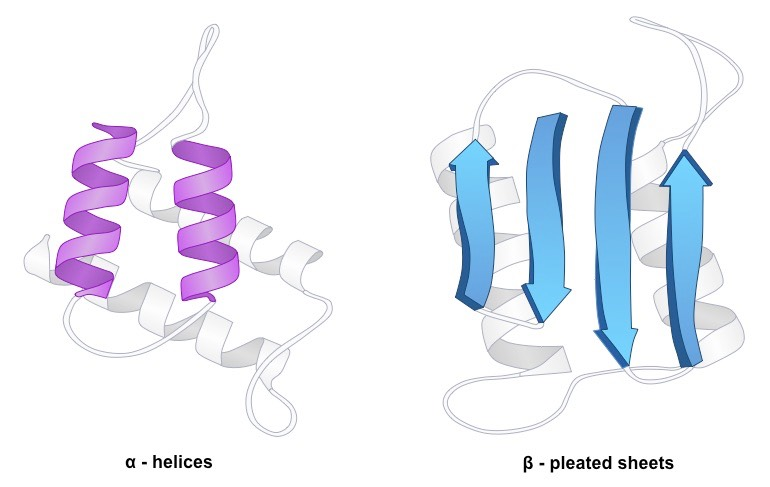
\includegraphics[scale=0.4]{images/secondary.jpeg}
	\caption{Struttura secondaria delle proteine, $\alpha$-eliche e $\beta$-foglietti. Fonte: \cite{proteinStrucBioNinja}}
	\label{fig:struttura-secondaria}
\end{figure}

Questo livello di organizzazione è una conseguenza dei legami a idrogeno intramolecolari. All'interno della backbone del polipeptide gli atomi di ossigeno hanno una parziale carica negativa e gli atomi di idrogeno attaccati all'azoto hanno una parziale carica positiva perciò possono formarsi legami idrogeno fra questi atomi. Individualmente sarebbero deboli legami ma poiché sono ripetuti molte volte su di una regione relativamente lunga di una catena polipeptidica possono fare da supporto per una particolare conformazione.

\par Nella struttura ad $\alpha$-elica, la struttura secondaria più comune e teorizzata già negli anni '50 da Linus Pauling, gli amminoacidi sono avvolti in una spirale tenuta insieme da legami idrogeno ogni 4 amminoacidi. Tra l’atomo di idrogeno legato all’azoto di ogni legame peptidico e l’ossigeno del gruppo carbossilico del legame peptidico sovrastante (che si trova a distanza di tre amminoacidi lungo la catena) si instaura un legame a idrogeno. Tuttavia se gli amminoacidi che si succedono lungo un tratto di catena proteica hanno gruppi R voluminosi, come avviene nella prolina, o gruppi R dotati della stessa carica elettrica, come avviene negli amminoacidi lisina e arginina, l’$\alpha$-elica non può formarsi, a causa delle forze di repulsione che si generano tra i residui. Alcune proteine fibrose, come l'$\alpha$-cheratina, la proteina strutturale di capelli, lana e unghie hanno formazioni di $\alpha$-eliche sulla maggior parte della loro lunghezza.

\begin{figure}[!htb]
	\minipage{0.5\textwidth}
	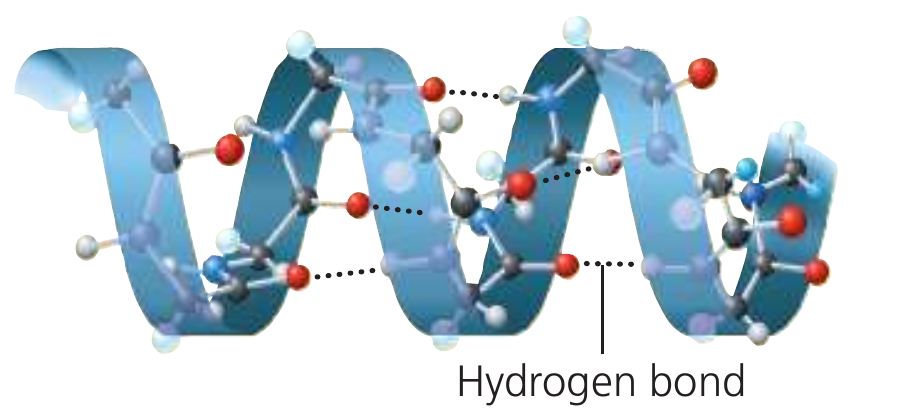
\includegraphics[scale=0.34]{images/eliche.png}
	\caption{Regione di $\alpha$-elica. Fonte: \cite{campbell}}
	\label{fig:eliche}
	\endminipage\hfill
	\minipage{0.5\textwidth}
	\centering
	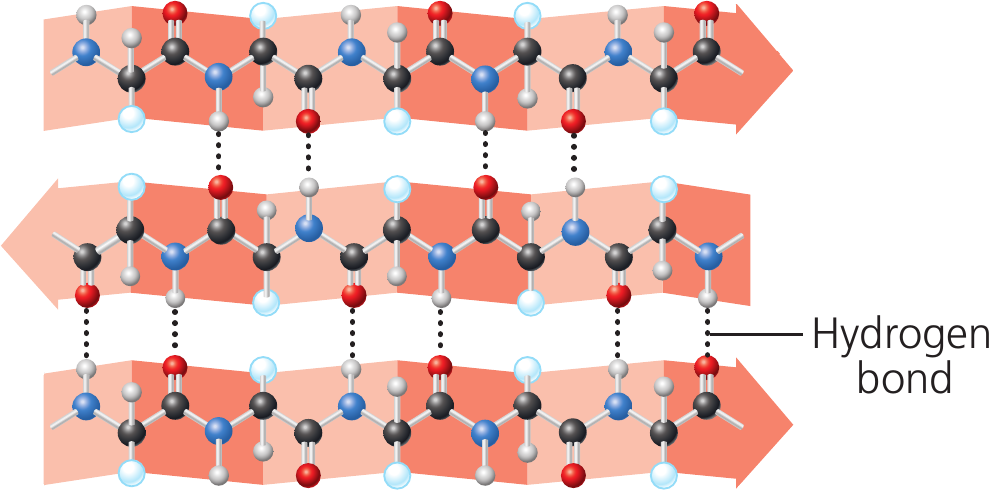
\includegraphics[scale=0.31]{images/foglietti.png}
	\caption{Una regione di $\beta$-foglietto composto da $\beta$-filamenti adiacenti, spesso mostrati come una freccia pieghettata o piatta puntata in direzione C-terminus. Fonte \cite{campbell}}
	\label{fig:foglietti}
	\endminipage\hfill
\end{figure}

Altre proteine fibrose sono invece dominate dai $\beta$-foglietti, come le proteine della seta ($\beta$-cheratina) e della tela prodotta dai ragni. In queste conformazioni due o più segmenti della catena polipeptidica giacenti lato su lato (chiamati $\beta$-filamenti) sono connessi da tre o più legami idrogeno. Si definisce $\beta$-filamento una sequenza peptidica di amminoacidi (tipicamente 5-10) che si dispone linearmente ed è in grado di formare legami idrogeno. Ciascuna delle catene è totalmente estesa e presenta una conformazione a zig-zag, dovuta alla geometria dei legami attorno a ciascun atomo di carbonio e di azoto nella catena.

\par  I gruppi amminici di uno scheletro peptidico formano legame con quelli carbossilici del filamento opposto. In ogni singolo filamento i residui si dispongono perpendicolarmente al piano del foglietto, puntando alternativamente verso l'alto e verso il basso. I $\beta$-foglietti tendono a trovarsi all'interno del nucleo della struttura per evitare competizione con le molecole d'acqua per formare legami idrogeno e tendono a favorire residui idrofobici. Si dice che i filamenti sono paralleli quando vanno nella stessa direzione (la freccia che indica la direzione C-terminus è puntata nella stessa direzione).


\par Nella vita quotidiana, se tiriamo per i due estremi una fibra di lana questa si allunga: si stanno rompendo i legami idrogeno e le eliche si allontanano sempre di più, ma lasciando la presa i legami idrogeno si riformano e le eliche ricompaiono nella struttura. Se invece tiriamo la seta si può osservare che non è elastica: i foglietti di cui è composta la sua struttura non sono smantellabili senza rompere anche i legami covalenti della backbone.

}
\subsubsection{Struttura supersecondaria}
{
La struttura supersecondaria è riferita alle combinazioni spaziali di strutture secondarie in conformazioni più complesse e alle connessioni che li uniscono\footnote{Non c'è un accordo tra i vari studiosi su di una precisa classificazione di questo livello strutturale.}. Può essere considerata come esempio di struttura supersecondaria la triplice elica allungata del collagene.

\begin{figure}[!htb]
	\minipage{0.5\textwidth}
	\centering
	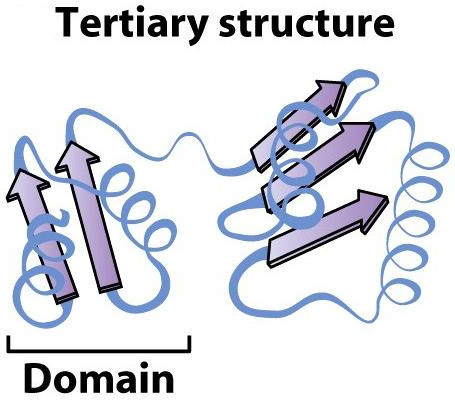
\includegraphics[scale=0.4]{images/dominio.jpg}
	\caption{Dominio in una proteina. Fonte: \cite{moran2012principles}}
	\label{fig:domini}
	\endminipage\hfill
	\minipage{0.5\textwidth}
	\centering
	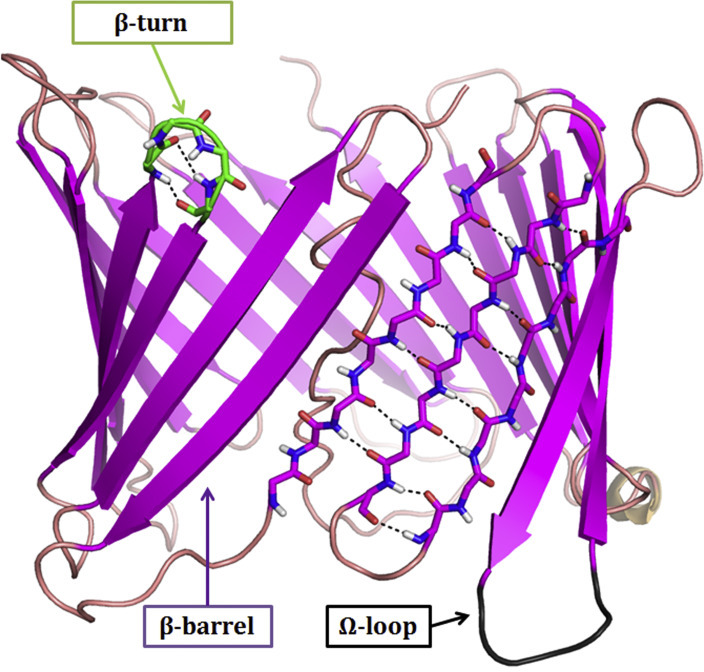
\includegraphics[scale=1]{images/turn-loop.jpg}
	\caption{Struttura con giri, loop e motivo $\beta$-barile. Fonte: \cite{MURRAY2017477}}
	\label{fig:turn-loops}
	\endminipage\hfill
\end{figure}

\par I \textit{motivi} (motifs) e \textit{domini} (domains) sono regioni tridimensionali della catena polipeptidica formate da differenti strutture secondarie adibite a svolgere una determinata funzione per la proteina di cui fanno parte. Tuttavia sono differenti in quanto i motivi non mantengono la loro forma se separati dalla proteina laddove i domini la mantengono. Questo perché i motivi e il resto della proteina sono più vicini e si vengono così a formare legami idrogeno che permettono ai motivi di mantenere la struttura. I domini sono sì legati alla backbone della proteina ma non abbastanza vicini alla restante parte della formazione proteica da stabilire legami, pertanto se vengono separati non perdono la loro struttura e possono mantenere la loro funzione. Una proteina con vari domini può usare questi per interazioni funzionali con differenti molecole.

\par Più in generale un \textit{motivo strutturale} è una struttura tridimensionale comune che appare in una varietà di molecole differenti ed evoluzionisticamente scollegate. Nel contesto delle sequenze amminoacidiche si definisce \textit{motivo} un pattern amminoacidico conservato in un gruppo di proteine con attività biochimica simile.

\begin{figure}[!htb]
	\minipage{0.5\textwidth}
	\centering
	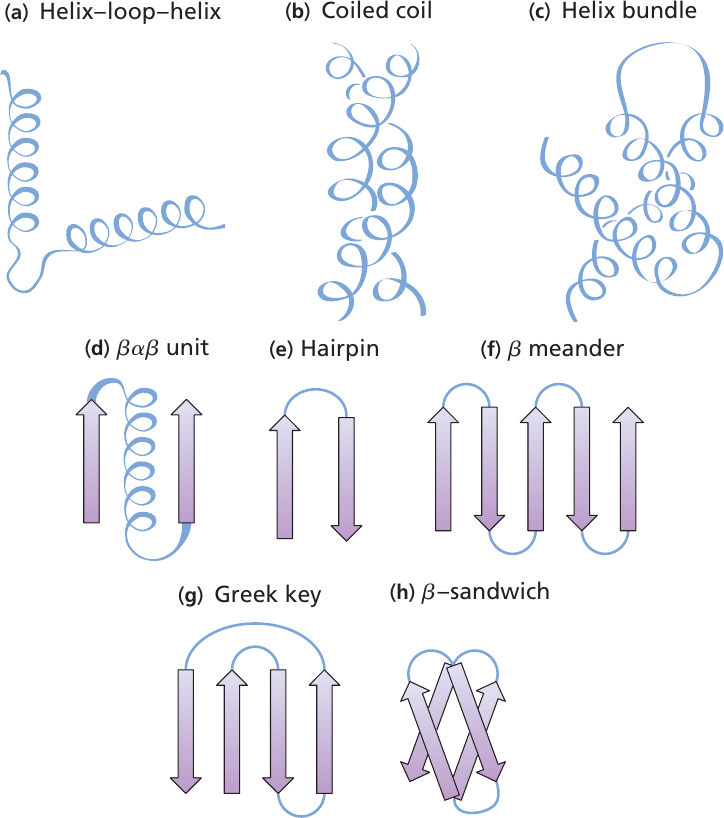
\includegraphics[scale=0.4]{images/motivi-comuni.png}
	\caption{Motivi comuni. Fonte \cite{moran2012principles}}
	\label{fig:motivi-comuni}
	\endminipage\hfill
	\minipage{0.5\textwidth}
	\centering
	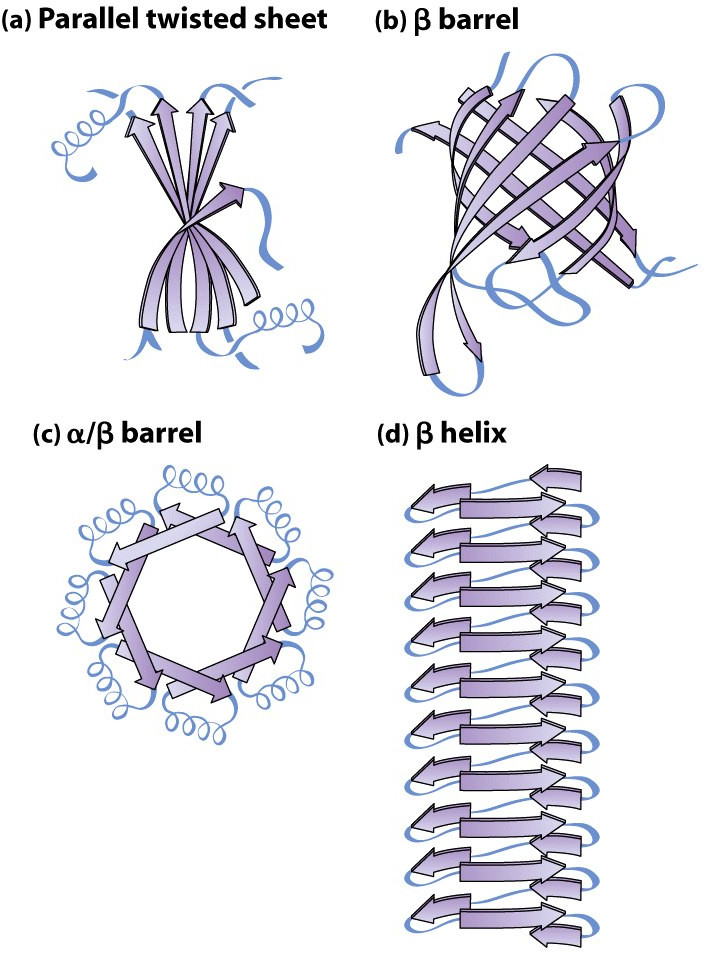
\includegraphics[scale=0.5]{images/domain-folds.jpg}
	\caption{\textit{Domain folds} (ripiegamenti di dominio). Fonte: \cite{moran2012principles}}
	\label{fig:domain-folds}
	\endminipage\hfill
	
\end{figure}

\par In figura \ref{fig:motivi-comuni} sono illustrati alcuni motivi comuni nelle strutture proteiche. 
Il motivo \textit{elica-loop-elica} ad esempio consiste di due $\alpha$-eliche collegate da un giro invertito. Un motivo simile è l'\textit{elica-giro-elica} dove al posto di un loop si ha un giro che causa un cambio di direzione più netto. Questa particolare conformazione rende questo motivo in grado di legarsi alla scanalatura del DNA e infatti questo motivo si presenta in molte proteine che regolano l'espressione genica.

\par Il motivo a \textit{simbolo greco} consiste di 4 $\beta$-filamenti antiparalleli in un $\beta$-foglietto dove l'ordine dei foglietti lungo la catena polipeptidica è 4,1,2,3\footnote{I numeri indicano l'ordine dei filamenti ovvero la loro posizione nel $\beta$-foglietto da destra a sinistra.}. In figura \ref{fig:turn-loops} e \ref{fig:domain-folds} è illustrato il motivo $\beta$-barile composto da $\beta$-foglietti ripiegati circolarmente a formare una struttura somigliante ad un barile comune in molte proteine di membrana. I \textit{domain folds}, o ripiegamenti di dominio, sono grandi motivi che costituiscono il nucleo di un dominio.

\par \textit{Giri} e \textit{loop} causano cambi di direzione alla backbone della proteina. I loop sono regioni con una struttura tridimensionale fissa ma non regolare. Si trovano generalmente sulla superficie delle proteine. Non sono strutture casuali e non vanno confuse con regioni disordinate o dispiegate. Una loro funzione è di connettere strutture secondarie tra loro. I loop sono regioni con ruoli spesso cruciali (interazioni con altre proteine, siti di legame con molecole ecc.) ma sono anche molto variabili nella loro sequenza e struttura. È stato ipotizzato che la posizione degli introni nel DNA possa correlare con la locazione dei loop codificati nella proteina\supercite{PSPwiki}.

\par Nelle strutture secondarie e terziarie si trovano spesso bruschi cambiamenti di direzione nella struttura: i \textit{giri} (turns). Queste nette svolte sono possibili grazie agli amminoacidi prolina e glicina. Il gruppo R della prolina si ripiega verso il gruppo amminico, distorcendo la catena naturalmente. Si forma però uno stretto spazio a causa del giro: l'amminoacido con gruppo R meno voluminoso è ovviamente la glicina ed è per questo che si trovano insieme nei giri.

}
\subsubsection{Struttura terziaria}
{
La struttura terziaria è la struttura tridimensionale globale risultante dalle interazioni tra i residui successivamente alle conformazioni locali della struttura secondaria ed è quindi la descrizione del risultato del processo di ripiegamento proteico. Un tipo di interazione importante è quella idrofobica che induce i residui non polari (e quindi idrofobici) a raggrupparsi al centro della catena polipeptidica, formando un \textit{nucleo idrofobico}. La forma della proteina può venire rinforzata dai ponti disolfuro, legami covalenti possibili solamente fra due cisteine.

\begin{figure}[!htp]
	\centering
	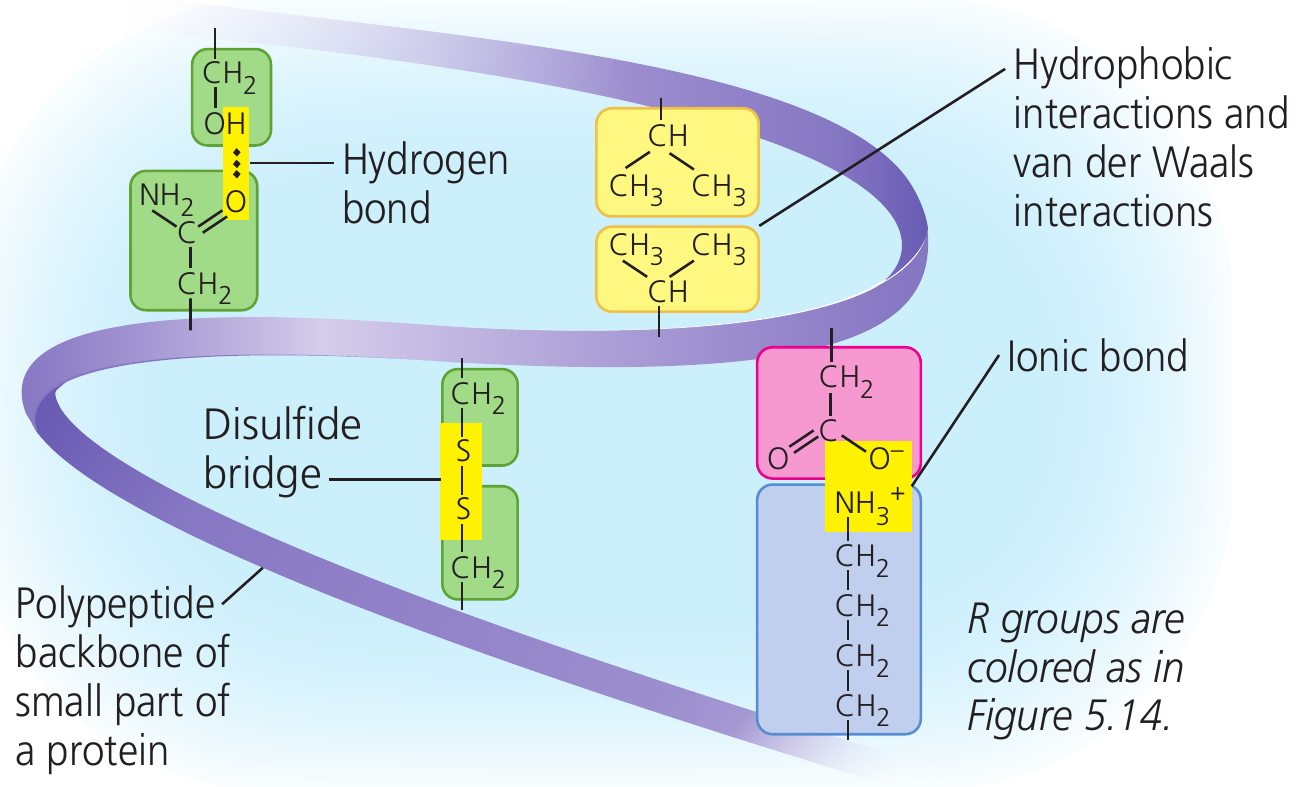
\includegraphics[scale=0.35]{images/interazioni-proteine.png}
	\caption{I diversi tipi di interazioni che possono contribuire alla struttura terziaria di una proteina. Fonte: \cite{campbell}}
	\label{fig:interazioni-proteine}
\end{figure}

La glicina assume una speciale posizione tra gli amminoacidi dato che ha il gruppo R più piccolo, un solo atomo di idrogeno (vedi fig. \ref{fig:amminoacidi-tipi}): può aumentare la flessibilità locale nella struttura (come infatti accade nel caso dei \textit{giri} sopra accennati). 

\par Prima degli anni '80 il protein folding code (bilancio termodinamico delle forze interatomiche, vedi sez. \ref{sec:problema-protein-folding}) era visto come la somma di molte piccole interazioni (legami idrogeno, interazioni di van der Waals, attrazioni elettrostatiche) ma senza nessuna forza dominante\supercite{dill2008protein}. Negli anni '80, grazie alla modellazione basata sulla meccanica statistica, è emerso un nuovo paradigma: la componente dominante nel folding code sono le forze idrofobiche, il folding code è distribuito sia localmente che non localmente nella sequenza e le strutture secondarie di una proteina sono una conseguenza della struttura terziaria tanto quanto una causa. Poiché le strutture native sono solamente 5-10kcal/mol più stabili dei loro stati denaturati è chiaro che nessuna forza intermolecolare può essere ignorata, e per questo la questione su quale forza sia quella dominante non è né semplice né risolta. Tuttavia risulta evidente che solo pochi residui risultano carichi nelle proteine, pertanto le forze elettrostatiche difficilmente possono essere dominanti. 

\begin{figure}[!htb]
	\centering
	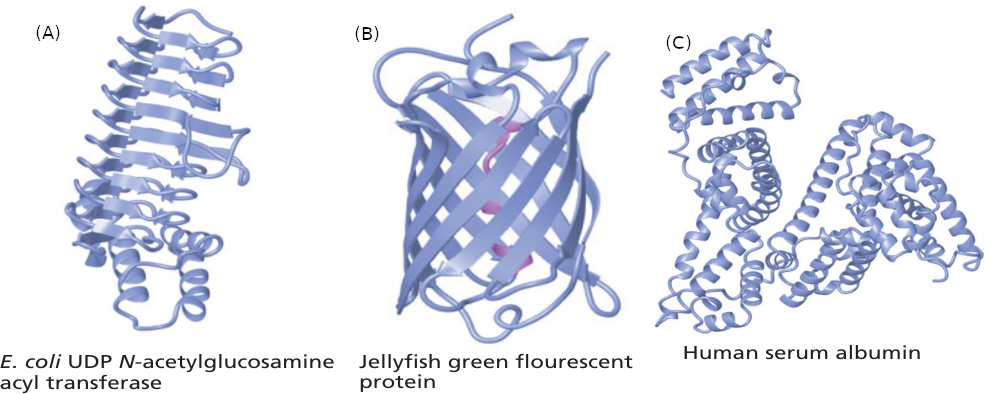
\includegraphics[scale=0.6]{images/strutture-proteine-complesse.png}
	\caption{Esempi di strutture terziarie in alcune proteine. (A) (classe: all-$\beta$) La struttura dell'enzima mostra un classico esempio di $\beta$-eliche, struttura abbastanza rara. (B) (classe: all-$\beta$) Struttura a $\beta$-barile con un'$\alpha$-elica centrale; i $\beta$-filamenti sono anti-paralleli. (C) (classe: all-$\alpha$)  Albumina del siero umano. Ha molti domini costituiti da $\alpha$-eliche a strati e helix bundle. Fonte \cite{moran2012principles}}
	\label{fig:strutture-complesse}
\end{figure}

}
\subsubsection{Struttura quaternaria}
{
\begin{figure}[!htb]
	\centering
	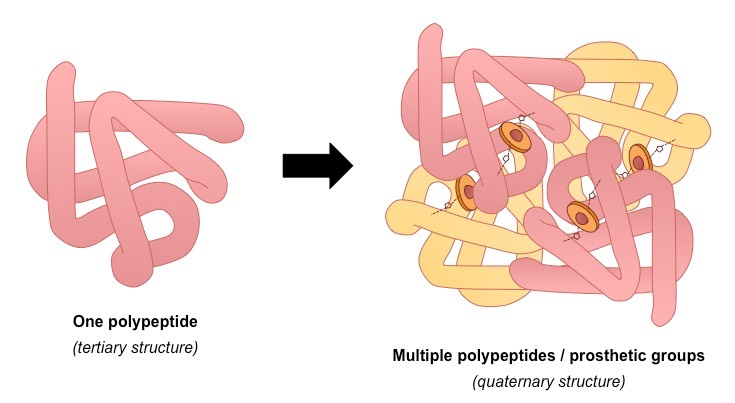
\includegraphics[scale=0.35]{images/quaternary-structure_med.jpeg}
	\caption{Rappresentazione di una struttura quaternaria composta da più polipeptidi e alcuni gruppi prostetici. Fonte \cite{proteinStrucBioNinja}}
	\label{fig:struttura-quaternaria}
\end{figure}

La struttura quaternaria è la forma finale di proteine "assemblate" da 2 o più catene polipeptidiche già ripiegate. Il collagene ne è un esempio poiché è formata da 3 polipeptidi quasi interamente a spirale che si attorcigliano l'uno sull'altro formando un'elica tripla ancora più larga, dando alle lunghe fibre una grande forza (vedi anche la cheratina nella sezione \ref{sec:classificazione}). Un altro esempio è l'emoglobina, proteina globulare formata da 4 subunità polipeptidiche. Le strutture terziarie delle subunità non vengono alterate.

\begin{figure}[!htb]
	\centering
	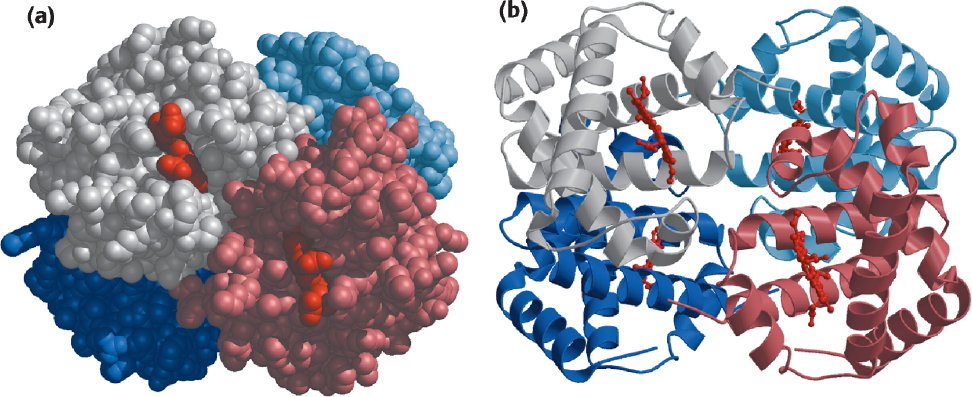
\includegraphics[scale=0.5]{images/quate-deossi.png}
	\caption{Struttura quaternaria della deossiemoglobina, ogni colore rappresenta una diversa subunità. (A) rappresentazione di tipo space-fill. (B) Rappresentazione a nastro. Fonte \cite{moran2012principles}}
	\label{fig:quate-deossi}
\end{figure}

La struttura che ne risulta è spesso chiamata \textit{oligomero} e le catene polipeptidiche costituenti sono dette \textit{monomeri}, \textit{protomeri} o \textit{subunità}. Le subunità sono unite mediante legami idrogeno, ionici o forze idrofobiche. I rapporti spaziali tra le subunità sono fissi e la geometria della molecola globale è ben definita.
L'unione delle subunità può far emergere proprietà non possedute dai singoli monomeri.
}
\subsection{Evoluzione e classificazione}
{
\subsubsection{Evoluzione e conservazione}
L’evoluzione degli organismi è legata a mutazioni spontanee che avvengono nei loro geni. Le differenze nella struttura primaria sono la “memoria” dei cambiamenti avvenuti a livello genetico nel corso dell’evoluzione. In specie legate da notevole affinità le strutture primarie delle proteine comuni sono
simili. Proteine con funzioni analoghe presentano sequenze simili, è molto probabile quindi che queste sequenze si siano evolute a partire da un progenitore comune. 

\par Al contrario di quanto si possa credere la maggior parte dei \textit{motivi} non ha origini evolutive in comune. Motivi simili sono sorti indipendentemente e semplicemente convergono verso una struttura stabile comune. Il fatto che gli stessi motivi si presentino in centinaia di differenti strutture suggerisce l'esistenza di un numero limitato di possibili ripiegamenti nell'universo delle strutture proteiche\supercite{proteinMotifs}. 

\subsubsection{Classificazione} \label{sec:classificazione}
La classificazione delle proteine all'interno dei database può essere basata su somiglianze strutturali e/o di sequenza. A livello biologico, in base ai diversi livelli strutturali assunti, le proteine sono classificate in \textit{fibrose} e \textit{globulari}.

\par Le proteine fibrose sono caratterizzate dalla prevalenza di strutture secondarie rispetto a livelli di organizzazione superiore. Sono costituite da lunghe catene disposte in lunghi fasci o foglietti. La struttura è estremamente ordinata. Svolgono funzioni di protezione e sostegno. Le proteine fibrose costituiscono prevalentemente: pelle, piume, capelli, corna, unghia, squame (con funzione di protezione) e cartilagine, tendini, ossa (con funzione di sostegno). Contengono per la maggior parte residui idrofobici, pertanto le proteine fibrose risultano insolubili in acqua. Esempi di proteine fibrose sono: cheratina, collagene, elastina, fibroina. 

\par In figura \ref{fig:capello} è mostrata la struttura di un capello. La proteina dei capelli è l'$\alpha$-cheratina, una struttura totalmente ad $\alpha$-eliche. Un paio di queste eliche si attorcigliano per formare una doppia elica. Queste si combinano poi in strutture di ordine superiore chiamate \textit{protofilamenti} e successivamente \textit{protofibrille}. Circa 4 fogli di protofibrille ($4\times2^{3}=32$ eliche di $\alpha$-cheratina in tutto) si combinano per formare un filamento intermedio. Un capello è una schiera di filamenti intermedi di $\alpha$-cheratina.

\begin{figure}[h]
	\centering
	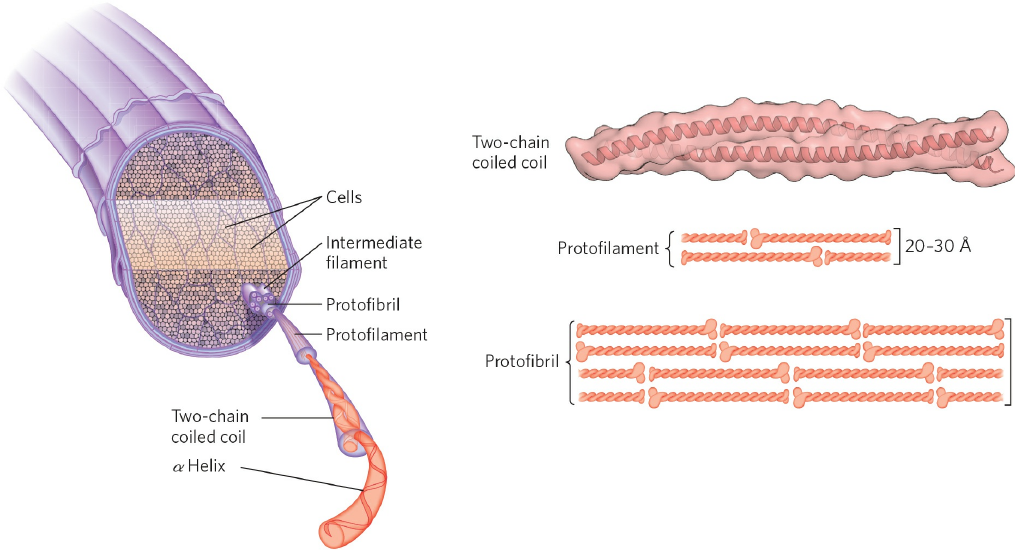
\includegraphics[scale=0.6]{images/capello-full.png}
	\caption{Struttura di un capello. Fonte: \cite{nelson2017lehninger}}
	\label{fig:capello}
\end{figure}

Le proteine \textit{globulari} assumono una struttura terziaria e a volte quaternaria. Sono macromolecole compatte di forma all'incirca sferica. Hanno una struttura meno ordinata rispetto a quelle fibrose. Svolgono funzioni di catalisi, trasporto e regolazione di processi cellulari. Categorie di proteine globulari sono: enzimi, trasportatori di ossigeno e lipidi, alcuni ormoni, recettori di membrana e anticorpi. La struttura è caratterizzata da brevi tratti di $\alpha$-elica e struttura $\beta$, collegate da tratti non organizzati in struttura secondaria. Sono proteine solubili nel citosol. 

}
}

\section{Dinamica del ripiegamento} \label{sec:assisted-folding}
{
{	
\subsection{Geometria ed energetica del ripiegamento}
{
	
\subsubsection{Geometria del ripiegamento}
Le tante conformazioni possibili della catena polipeptidica sono possibili grazie alla rotazione di essa attorno all'atomo $C_{\alpha}$ di ogni amminoacido.

\begin{figure}[!htb]
	\centering
	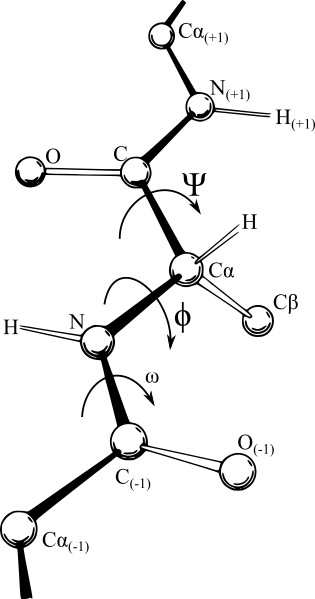
\includegraphics[scale=0.4]{images/angoli-torsione.png}
	\caption{Angoli di torsione intorno all'atomo $C_{\alpha}$}
	\label{fig:angoli-torsione}
\end{figure}

I tre angoli di torsione principali di un polipeptide sono $\phi$, $\psi$ ed $\omega$; i legami N-$C_{\alpha}$ e $C_{\alpha}$-C sono relativamente liberi nella rotazione (angoli $\phi$ e $\psi$), mentre il legame N-C ($\omega$) è fisso dato il carattere di doppio legame parziale del legame peptidico alle temperature fisiologiche.

\par Data la relativa libertà dei due legami si ha la possibilità di isomeria: le due configurazioni possibili sono \textit{cis } e \textit{trans}. Delle due configurazioni possibili, la trans è quella favorita dal punto di vista
energetico (minima repulsione sterica), infatti oltre il 99\% dei legami peptidici delle proteine naturali hanno configurazione trans.

\subsubsection{Grafico di Ramachandran}

\begin{figure}[!htb]
	\centering
	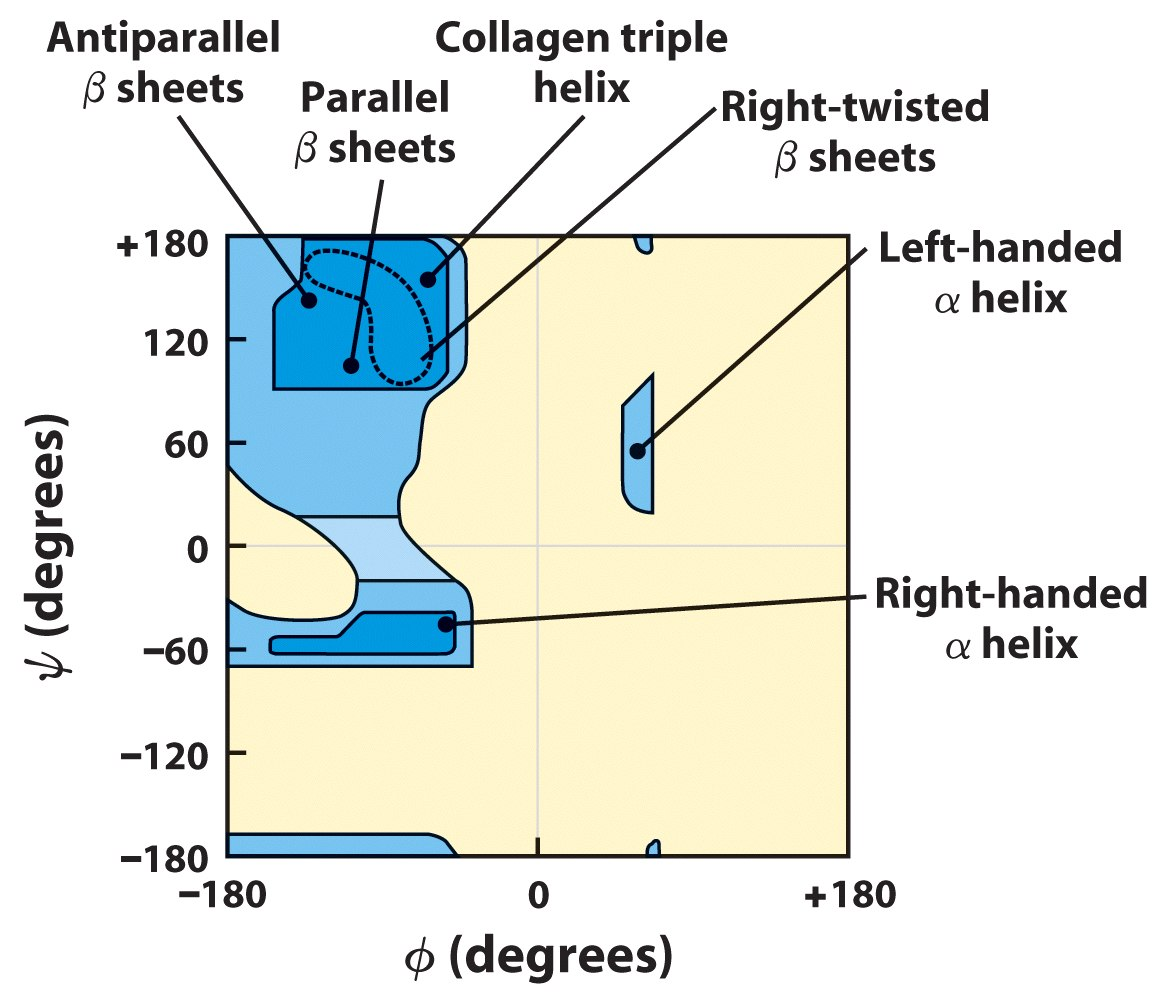
\includegraphics[scale=0.4]{images/Ramachandran's_Diagram.jpg}
	\caption{Grafico di Ramachandran. Fonte \cite{ramachandranDiag}}
	\label{fig:ramachandran}
\end{figure}

Nel \textit{grafico di Ramachandran} sono riportati in ordinata i valori di Ψ ed in ascissa i valori di Φ. Ogni puntino (non presenti in figura) rappresenta la posizione di un residuo. Il grafico deriva da un modello in cui è simulata la variazione di struttura di piccoli polipeptidi e successivamente si cercano conformazioni stabili. Per ciascuna conformazione sono esaminati i contatti tra atomi, trattati come sfere solide di dimensioni determinate dai raggi di van der Waals. Le conformazioni non consentite sono quelle per le quali sono previste collisioni tra sfere. In figura \ref{fig:ramachandran} l'area giallina corrisponde a conformazioni instabili in cui atomi della catena sono ad una distanza inferiore alla somma dei raggi di van der Waals. Tali regioni sono stericamente non consentite per tutti gli aminoacidi, fatta eccezione per la glicina, priva di catena laterale. Le regioni blu indicano conformazioni consentite ($\beta$-foglietti e $\alpha$-eliche destrogire). Le aree azzurre mostrano le regioni consentite riformulando i calcoli con raggi di van der Waals più corti, ovvero consentendo una prossimità atomica maggiore.

\par Conformazioni ideali (in cui non vi sono interazioni tra catene laterali):
\begin{itemize}
	\item $\alpha$-elica: Φ= -57°, Ψ= -47°
	\item $\beta$-parallelo: Φ= -119°, Ψ= +113°
	\item $\beta$-antiparallelo: Φ= -139°, Ψ= +135°
\end{itemize}

\par In conformazioni diverse, c’è un limite al numero delle combinazioni
possibili dei due angoli di rotazione, perché alcune hanno effetti
destabilizzanti a causa delle forze di repulsione tra gli O. Vi sono quindi conformazioni più stabili di altre perché favorite da un
punto di vista energetico. Conformazioni proibite sono anche quelle in cui si svilupperebbe una forte repulsione tra le catene laterali.
}

\subsubsection{Energetica del ripiegamento} \label{sec:energetica}
La termodinamica caratterizza gli stati in natura dalla dipendenza da temperatura, pressione, volume e concentrazione chimica. 

\par L'entropia è la quantità di disordine di un sistema, in altri termini è il numero di possibili stati configurazionali del sistema ($\Omega$). 

\[ S = K_{B}ln{\Omega} \]

Nei sistemi molecolari cambiamenti di entropia ($\Delta S$) rappresentano cambiamenti nella libertà di movimento di atomi appartenenti sia al soluto che al solvente.  L'entalpia è l'energia interna al sistema. Cambiamenti positivi di entalpia nelle macromolecole sono associate alla rottura di interazioni non covalenti favorevoli (si assume che i legami covalenti restino invariati). La formazione di legami covalenti diminuisce l'entalpia del sistema e rilascia calore verso l'ambiente. Formando legami si libera energia mentre per romperli si consuma energia.

\[ \Delta H \simeq \Delta E \] 
\[ E = U + K \]

Dove H è l'entalpia, E l'energia interna al sistema, U l'energia potenziale (circa la somma di tutte le interazioni covalenti e non covalenti, ma non quelle non polari) e K l'energia cinetica (associata ai movimenti atomici indotti termicamente).\\

\par L'energia libera di Gibbs (G) è l'\textit{energia utile} sotto temperatura e pressione costante. I processi spontanei raggiungono l'equilibrio decrementando la G del sistema a un minimo.

L'energia libera di Gibbs è associata all'entropia e all'entalpia dalla seguente relazione:

\[ \Delta G = \Delta H - T \Delta S \]

\par La seconda legge della termodinamica afferma che in un sistema isolato i processi spontanei raggiungono l'equilibrio incrementando l'entropia del sistema. 

\par Il ripiegamento delle proteine è un processo spontaneo. Esibisce una grande varietà di percorsi, meccanismi e velocità che dipendono da parametri come la composizione della proteina e le condizioni di ripiegamento. A prescindere dall'esatto meccanismo, il processo di ripiegamento segue sempre la teoria del profilo energetico (a imbuto, \textit{energy landscape theory}), cioè il ripiegamento è sempre accompagnato da una decrescita del numero di conformazioni che possono essere testate dalla proteina, sfuggendo al paradosso di Levinthal (vedi sez. \ref{sec:problema-protein-folding}).

\par Una proteina che si ripiega deve procedere da uno stato ad alta energia ed alta entropia a uno stato caratterizzato da bassi valori di energia ed entropia;
tale nesso è conosciuto come \textit{imbuto di ripiegamento} (folding funnel, vedi fig. \ref{fig:imbuto}). 

\par Le forze idrofobiche causano la creazione del nucleo idrofobico seppellendo i residui non polari nella struttura nativa, questo vuol dire che l'entropia del solvente acquoso subisce un aumento portando ad una sovra compensazione dell'entropia, ovvero l'entropia del sistema aumenta.

\par Le proteine non cercano una conformazione fra tutte le possibili conformazioni fino a trovare quella giusta. Piuttosto si ripiegano in una maniera cooperativa in cui ogni step limita ulteriormente le possibilità di ripiegamento degli step seguenti. Il ripiegamento è completato quando la conformazione con più basso livello di energia libera associato alla proteina è trovata. La superficie rugosa del tunnel riflette il fatto che il processo di ripiegamento passi attraverso molti minimi locali separati da barriere da alta-energia. \\

\par Una visione più accurata della struttura nativa delle proteine (anche alla luce delle questioni alzate dalle IDP, vedi sez. \ref{sfide-dogma}) può essere la seguente: \\
\say{\textit{la struttura nativa di una proteina è quella conformazione avente minore energia libera tale da mantenere il livello di dinamicità richiesto alla proteina per svolgere la sua funzione biologica}\supercite{kessel_ben-tal_2018}}

\begin{figure}[!htb]
	\centering
	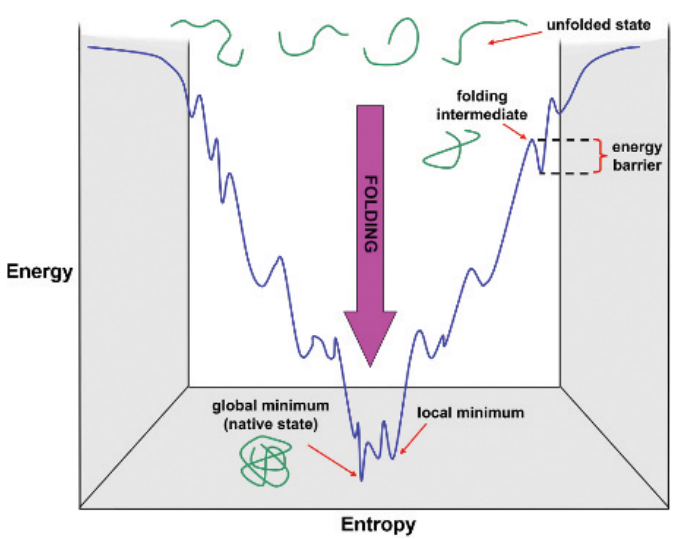
\includegraphics[scale=0.6]{images/imbuto.png}
	\caption{Profilo energetico a imbuto del ripiegamento. Fonte \cite{kessel_ben-tal_2018}}
	\label{fig:imbuto}
\end{figure}

Non c'è un meccanismo di ripiegamento universale, ma una collezione di possibili meccanismi che possono essere usati. La preferenza di una proteina ad usarne uno piuttosto che un altro può dipendere da vari fattori, uno dei quali sembra essere la struttura secondaria. Ad esempio in proteine dominate da $\alpha$-eliche il ripiegamento è spesso gerarchico. 

\par La velocità di ripiegamento correla non solo con la dimensione della proteina ma anche con la sua topologia nativa. Le proteine \textit{fast-folding} (ripiegamento su scala temporale di nanosecondi) tendono ad avere grandi proporzioni di elementi secondari locali ($\alpha$-eliche e giri) laddove quelle \textit{slow-folding} tendono ad avere proporzioni più grandi di elementi globali ($\beta$-foglietti).

\subsubsection{Termodinamica delle forze idrofobiche} \label{sec:termodinamica-forze-idrofobiche}

\par I fattori termodinamici che danno luogo all’effetto idrofobico sono complessi e non del tutto conosciuti. L’effetto idrofobico è visto come una combinazione dell’effetto di idratazione (effetto entropico) e di interazioni di van der Waals tra molecole di soluto (effetto entalpico). Le forze idrofobiche non scaturiscono da classiche interazioni atomo-atomo ma sono un effetto indiretto risultante dalle proprietà del solvente. Per questa ragione è stato difficile conoscere la vastità delle interazioni non polari, sebbene queste siano correlate con la dimensione delle molecole interagenti\supercite{kessel_ben-tal_2018}:
\begin{itemize}
	\item per piccole molecole ($<20$) atomi di carbonio), l'energia libera delle interazioni non polari correla con il numero di atomi di carbonio 
	\item per molecole più grandi come le proteine, l'energia libera correla l'area di superficie ($\Delta S$) della molecola:
	\[ \Delta G_{np} \approx -0.025\Delta SA \]
	ovvero per ogni $\angstrom^{2}$ della molecola interagente si ha un'energia libera di $\approx 25$ cal/mol.
\end{itemize}}

Questa relazione dimostra che ogni molecola con un'area di superficie può partecipare in interazioni non polari. Dato che molte molecole includono gruppi polari e hanno un'estesa area di superficie è il bilancio tra i due tipi di interazione (polare e non polare) che determina la tendenza complessiva della molecola ad essere \textit{idrofila} o \textit{idrofobica}.

}
	
\subsection{Ripiegamento assistito}
All'interno delle cellule le proteine più piccole si ripiegano indipendentemente, mentre proteine più grandi sono assistite principalmente da complessi chiamati \textit{chaperoni molecolari}. È  importante notare che l'assistenza è cinetica in natura: non aggiunge nuove informazioni necessarie alla proteina per ripiegarsi, pertanto il dogma di Anfinsen non viene contraddetto. Ciò che fanno questi complessi è creare un ambiente nel quale le proteine possano ripiegarsi senza "distrazioni" dovute a interazioni con altre entità (ad esempio evitando l'aggregazione con altre proteine) e senza rimanere bloccate in conformazioni intermedie durante il loro percorso di ripiegamento. In poche parole sono misure di protezione della cellula. 

\begin{figure}[h]
	\centering
	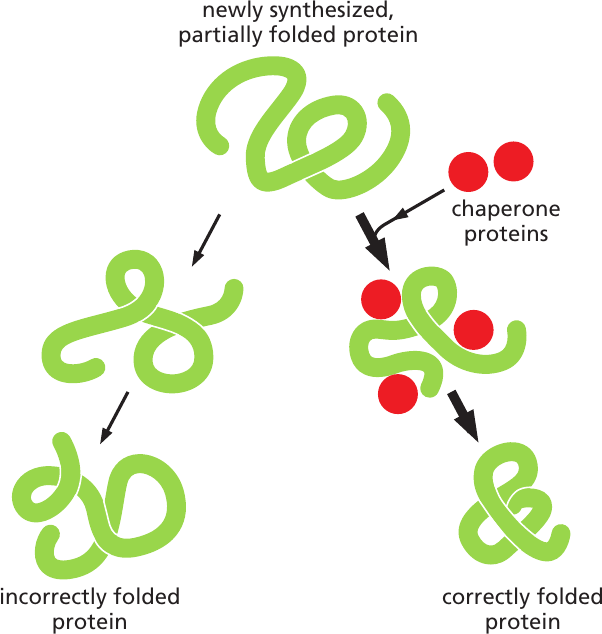
\includegraphics[scale=0.4]{images/chaperone-alberts.png}
	\caption{Schema della funzione dei chaperoni molecolari. Fonte: \cite{alberts2018essential}}
	\label{fig:chaperoni}
\end{figure}

Più in dettaglio i chaperoni molecolari svolgono le seguenti funzioni:
\begin{enumerate}
	\item assistono il corretto ripiegamento delle catene polipeptidiche (lunghe) appena sintetizzate
	\item dirigono l'assemblaggio di complessi multi-enzimatici
	\item donano una "seconda chance" a proteine danneggiate favorendone la rinaturazione
	\item partecipano nella parziale denaturazione durante il trasporto di proteine attraverso membrane di mitocondri o cloroplasti
\end{enumerate}

Tutti i compartimenti cellulari delle cellule eucariotiche (nucleo, citosol, reticolo endoplasmatico, mitocondri e cloroplasti) hanno il proprio set di chaperoni che assicura un corretto ripiegamento delle proteine. I chaperoni molecolari comprendono diverse famiglie di proteine altamente conservate, tra cui le Hsp (Heat shock protein), proteine espresse in grande quantità sotto condizioni di alto stress, per contrastarne l'effetto denaturante. Queste ultime sono state classificate in base al loro peso molecolare, ad es. Hsp60 dove "60" indica 60kDa. Le Hsp60 vengono chiamate anche \textit{chaperonine} e sono una famiglia di chaperoni molecolari a doppio anello che agiscono da "camera di isolamento" per il ripiegamento di altre proteine\supercite{ranson1998chaperonins}, famosa è la chaperonina procariotica GroEL (vedi fig. \ref{fig:groel}), che può essere assunta come modello di riferimento delle chaperonine. 

\begin{figure}[h]
	
\end{figure}

\begin{figure}[!htb]
	\minipage{0.35\textwidth}
	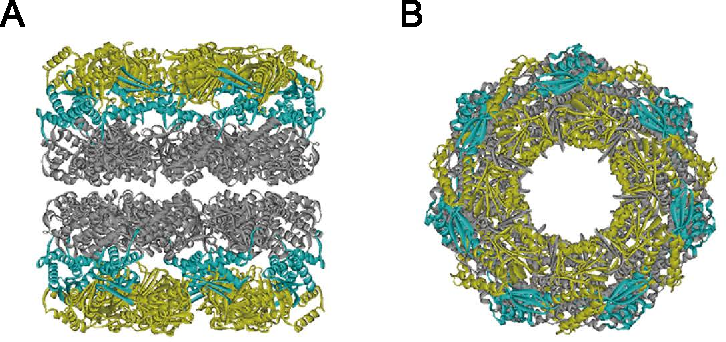
\includegraphics[scale=0.25]{images/groel.png}
	\caption{Strutture dei complessi GroEL e GroEL-GroES. (B) si può osservare la tipica forma ad anello. Fonte: \cite{Iizuka2016ChaperoninGU}}
	\label{fig:groel}
	\endminipage\hfill
	\minipage{0.6\textwidth}
	\centering
	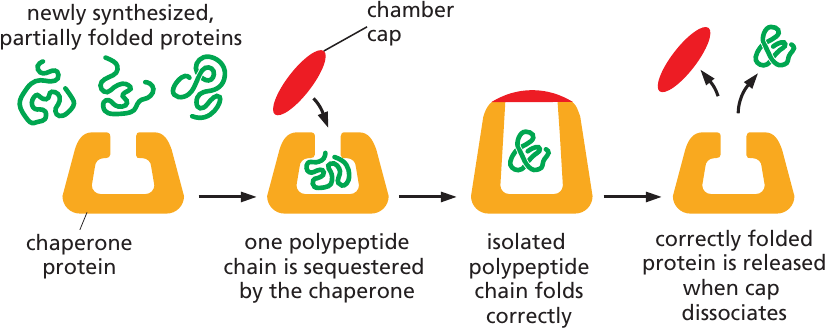
\includegraphics[scale=0.4]{images/chaperone-alberts-isolation.png}
	\caption{Rappresentazione schematica della funzione della camera di isolamento nelle chaperonine. Fonte \cite{alberts2018essential}}
	\label{fig:chaperone-camera}
	\endminipage\hfill
\end{figure}

Sebbene i mitocondri (e i cloroplasti) abbiano il loro genoma e creino le loro proteine, la maggior parte delle proteine che questi organelli usano sono codificate dai geni nel nucleo e importati dal citosol. Ogni proteina viene quindi parzialmente denaturata per effettuare il trasporto. I chaperoni molecolari all'interno di questi organelli aiutano a tirare le proteine attraverso le due membrane e a ripiegarle una volta all'interno\supercite{alberts2018essential}.


\subsection{Misfolding, prioni e malattie}
{
	
\subsubsection{Misfolding}
Il \textit{misfolding} è il fenomeno dell'errato ripiegamento di una proteina, ovvero quando una proteina non può raggiungere il suo stato nativo. Ciò può accadere per mutazioni alla sua sequenza amminoacidica (anche per un solo amminoacido differente come nel caso dell'anemia falciforme) o per fattori esterni. Le proteine mal ripiegate tipicamente contengono $\beta$-foglietti organizzati in una struttura denominata cross-$\beta$, disposizione molto stabile e insolubile, resistente alla proteolisi. Il mal ripiegamento di alcune proteine può innescare ulteriori mal ripiegamenti e la conseguente accumulazione di proteine mal ripiegate in aggregati (od oligomeri) che possono guadagnare tossicità attraverso le interazioni intermolecolari. L'incremento dei livelli di proteine aggregate può portare alla formazione di \textit{amiloidi}, strutture fibrillari formate da deposizioni di materiale proteico insolubile. 

\subsubsection{Malattie}
L'errato ripiegamento delle proteine è alla base quindi di molte patologie umane, definite malattie da misfolding, categorizzabili in due gruppi:

\begin{itemize}
	\item malattia causata dalla perdita o degradazione della proteina o dall'errato trasporto intracellulare
	\item malattie causate dall'accumulo, intra od extra-cellulare, di proteine aggregate (ad esempio le malattie da prione)
\end{itemize}

Molti tipi di tumore diventano chemio-resistenti perché iper-esprimono alcune Hsp, come la Hsp70 e la Hsp90. Le Hsp sono presenti anche in quantità elevatissime nel cervello dei pazienti con malattia di Alzheimer e morbo di Parkinson. Tuttavia si crede che la loro aumentata espressione non sia lesiva di per sé ma rappresenti piuttosto una risposta difensiva agli elevati livelli di stress che caratterizzano queste patologie. Ci sono molti morbi associati a mutazioni nei geni codificanti i chaperoni. Alterazioni genetiche delle chaperonine possono portare a patologie umane che in genere colpiscono molti organi ed apparati contemporaneamente \supercite{chaperoninaWiki}. \\


\subsubsection{Prioni}
\par I \textit{prioni} (acronimo di "\textbf{pr}oteinaceous \textbf{i}nfective \textbf{on}ly particle") sono molecole di natura proteica con la capacità di trasmettere la propria forma mal ripiegata a varianti normali della stessa proteina\footnote{I prioni sono stati studiati e denominati in questo modo dal premio Nobel per la medicina nel 1997 Stanley Prusiner\supercite{prusiner1998prion}.}. Il ruolo ipotizzato di una proteina come agente infettivo è in contrasto con tutti gli altri agenti infettivi conosciuti, come i viroidi, virus, batteri, funghi, parassiti: tutti contengono acidi nucleici (DNA, RNA o entrambi) mentre le proteine sono composte di soli amminoacidi.

\par I prioni formano amiloidi che si accumulano nei tessuti e sono associati a danni di questi e alla morte cellulare. I prioni sono attualmente considerati i più probabili agenti delle encefalopatie spongiformi trasmissibili (TSE) dei mammiferi. Nel \textit{morbo della mucca pazza} (encefalopatia spongiforme bovina), malattia neurologica degenerativa e irreversibile, vi è il ruolo di un prione a causare mal ripiegamenti di alcune proteine native causando la formazione di strutture amiloidi fatali (al microscopio le dense placche fibrose appaiono come buchi, da qui il caratteristico aspetto "a spugna"). Tutte le malattie da prione sono attualmente inguaribili e letali, con un periodo di incubazione che dura generalmente vari anni.

\par Gli aggregati di prioni sono stabili e questa stabilità strutturale consente loro di essere immuni alla maggior parte dei trattamenti conosciuti. L'organismo infettato non ha modo di degradarli: a differenza di virus e batteri i prioni rimangono intatti anche in presenza di trattamenti come sterilizzazione, forti dosi di radiazioni ionizzanti, uso di formaldeide, varechina, acqua bollente e a differenza delle altre proteine sono resistenti alla maggior parte delle proteasi.

\par La proteina di cui sono fatti i prioni, \textit{PrP} (protease-resistant-protein, Pr per \textbf{pr}ione, e P per \textbf{p}roteina), si trova in tutto il corpo, anche negli individui sani, ed è altamente conservata nei mammiferi. Tuttavia, la PrP trovata nel materiale infettante ha una struttura diversa. Nell'uomo la PrP$^{c}$(\textbf{c}ellulare, forma normale) è codificata da un solo gene, PRNP. La PrP$^{sc}$(\textbf{sc}rapie, forma patologica) differisce dalla proteina naturale PrP$^{c}$ per la conformazione tridimensionale: la PrP$^{c}$ ha una struttura più aperta contenente 3 segmenti ad $\alpha$-eliche e pochi $\beta$-foglietti; la PrP$^{sc}$ invece ha una struttura più compatta e stabile e presenta un aumento di $\beta$-foglietti.

\begin{figure}[h]
	\centering
	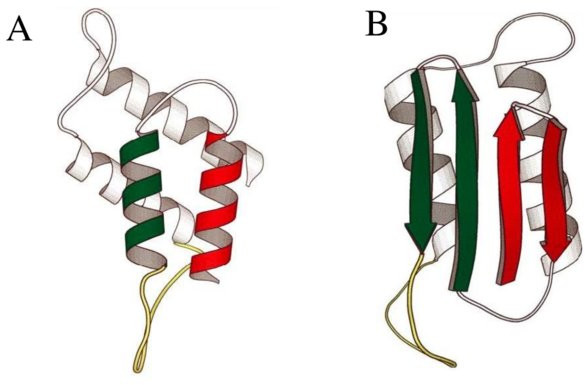
\includegraphics{images/PrPc.jpg}
	\caption{(A) Struttura della PrP$^{c}$. (B) Struttura della PrP$^{sc}$. Fonte: \cite{ruttkay2015prion}}
	\label{fig:PrPc}
\end{figure} 

}
\subsection{Controllo qualità e apoptosi}
{
\subsubsection{Controllo qualità}
L'uscita delle proteine dal reticolo endoplasmatico (RE) è controllata per assicurare la qualità delle proteine. Sebbene alcune siano appositamente create e destinate a funzionare nel RE la maggior parte delle proteine che entrano nel RE sono destinate ad altri luoghi. Queste vengono impacchettate nelle vescicole di trasporto e gemmano per fondersi con l'apparato del Golgi. Ma l'uscita dal RE è altamente selettiva: le proteine che falliscono a ripiegarsi nella forma nativa e quelle che non si assemblano correttamente sono attivamente conservate nel RE attraverso i legami con i chaperoni molecolari che risiedono lì. Questi trattengono le proteine nel RE finché non si verifica il corretto ripiegamento o assemblaggio. Se questo non si verifica o fallisce ancora le proteine sono esportate nel citosol dove sono degradate da un \textit{proteasoma}. Le proteine da degradare sono contraddistinte dal loro legame con l'ubiquitina\footnote{Per "la scoperta della degradazione delle proteine mediata da ubiquitina" è stato assegnato il Premio Nobel per la chimica del 2004.}.

\par Ad esempio gli anticorpi sono composti da 4 catene polipeptidiche che si assemblano in completi anticorpi nel RE. Gli anticorpi parzialmente assemblati sono conservati nel RE finché tutte e 4 le catene non sono pronte. Le molecole di anticorpi che falliscono ad assemblarsi vengono degradate.


\par Nonostante l'indubbia utilità di questo meccanismo di controllo a volte questo può rivelarsi dannoso per l'organismo. Ad esempio una classe di mutazioni che causa la \textit{fibrosi cistica}, comune malattia genetica che comporta seri danni polmonari, produce una proteina di trasporto della membrana plasmatica leggermente mal ripiegata. Tuttavia questa potrebbe funzionare normalmente se raggiungesse la membrana plasmatica ma, come viene suggerito da alcuni studi\supercite{fraser2015cystic}, viene bloccata nel RE e successivamente degradata\supercite{alberts2018essential} (per usare una metafora si può immaginare la situazione di un innocente condannato alla pena di morte). La nota da sottolineare in questo esempio specifico è che tale mutazione (una delle varie classi di mutazioni possibili nella fibrosi cistica) non causa un'inattivazione di una proteina importante ma la proteina attiva è scartata dalle cellule prima che questa possa avere l'opportunità di funzionare. \\

\subsubsection{Proteasomi}
\par I proteasomi sono complessi di \textit{proteasi} (enzima in grado di catalizzare la rottura del legame peptidico delle proteine) che 
degradano (principalmente) proteine anomale attraverso reazioni di \textit{proteolisi}. Sono presenti nelle cellule di tutti gli eucarioti e procarioti. La struttura e la funzione di questi complessi è altamente conservata.

\par A causa del ruolo dei proteasomi nella regolazione del ciclo cellulare e dell'apoptosi\footnote{Il termine \textit{apoptosi} indica una forma di morte cellulare programmata (un'auto-distruzione). Al contrario della necrosi, che è una forma di morte cellulare risultante da un acuto stress o trauma cellulare, l'apoptosi è portata avanti in modo ordinato e regolato, richiede consumo di energia (ATP) e generalmente porta a un vantaggio durante il ciclo vitale dell'organismo (è infatti chiamata da alcuni morte altruista o morte pulita). Durante il suo sviluppo, ad esempio, l'embrione umano presenta gli abbozzi di mani e piedi “palmati”: affinché le dita si differenzino, è necessario che le cellule che costituiscono le membrane interdigitali muoiano.}, sono oggi un bersaglio rilevante nelle terapie antitumorali. 

\par Le proteasi tuttavia possono anche essere utilizzate dai virus in maniera inversa, ovvero per produrre proteine, si parla di \textit{proteasi virali}\supercite{proteasiVirale}. Le proteine del \textit{core virale} vengono prodotte in lunghi filamenti polipeptidici, ognuno dei quali contiene varie copie di proteine del core. Le proteasi riconoscono specifiche sequenze poste fra una futura proteina e l'altra all'interno di queste catene ed effettuano dei tagli: le singole proteine vengono separate e possono quindi progredire nella loro maturazione, andando a costruire un core virale. 

\par Per fermare tale meccanismo sono stati progettati farmaci inibitori, specialmente nella terapia antiretrovirale (HIV, epatite C), che interferiscono con il ciclo replicativo del virus HIV proprio bloccando le proteasi. I filamenti polipeptidici non vengono più scissi se si inibisce l'attività di questi enzimi, non vengono più create le proteine del core e quindi gli stessi core. Senza core la replicazione virale si ferma.

}
\subsubsection{Unfolded protein response e Apoptosi}
{

La dimensione del RE è controllato dalla "richiesta" per il ripiegamento delle proteine. Il meccanismo di controllo nel RE, eseguito dai chaperoni molecolari, può essere sopraffatto. Quando succede le proteine mal ripiegate si accumulano nel RE. 
Se l'accumulo è abbastanza grande, questo innesca un complesso programma chiamato \textit{unfolded protein response} (UPR). Questo programma incita la cellula a produrre più RE, inclusi più chaperoni molecolari, e altre proteine riguardanti il controllo qualità. L'UPR permette alla cellula di regolare la dimensione del RE per gestire propriamente il volume delle proteine in entrata. In alcuni casi tuttavia anche un RE espanso non riesce a gestire la richiesta e l'UPR indirizza la cellula verso l'\textit{apoptosi}.

\par Una situazione del genere può avvenire negli adulti in cui insorge il diabete. I tessuti diventano gradualmente resistenti all'effetto dell'insulina. Per compensare questa resistenza le cellule che secernono insulina nel pancreas ne producono ancora di più. Si arriva infine alla situazione in cui il loro RE arriva ad una capacità massima e viene innescato l'UPR e di conseguenza la morte cellulare. Col tempo sempre più cellule secernenti insulina sono eliminate e la richiesta per quelle sopravvissute aumenta rendendole sempre più vulnerabili a questo meccanismo, esacerbando ulteriormente la malattia\supercite{alberts2018essential}.
}


\section{Studio sperimentale delle proteine} \label{sec:experimentally-guided-prediction}
{
	
	\subsubsection{Come vengono studiate le proteine}
	Comprendere come una particolare proteina funzioni richiede dettagli strutturali e analisi biochimiche: entrambe hanno bisogno di una grande quantità di proteine pure. Isolare però un singolo tipo di proteina dalle migliaia presenti in una cellula non è un compito semplice. Per molti anni le proteine sono state purificate direttamente dai tessuti nei quali esse erano abbondanti. Ciò comporta, oltre alla necessità fisica di procurarsi i tessuti, dover riconoscere le proteine da studiare. Queste procedure richiedono settimane e forniscono solamente pochi milligrammi di proteina pura. Oggi le proteine sono generalmente isolate da cellule coltivate in laboratorio e spesso queste sono modificate geneticamente al fine di produrre grandi quantità di una data proteina. \\
	
	\par Il primo step in una procedura di purificazione consiste nel rompere i tessuti e le cellule in modo da far loro rilasciare il contenuto (\textit{omogenizzazione}), chiamato \textit{estratto} (o omogenato cellulare). Ci sono vari meccanismi, come mostrato in fig. \ref{fig:break-cells}. 
	
	
	\begin{figure}[!htb]
		\centering
		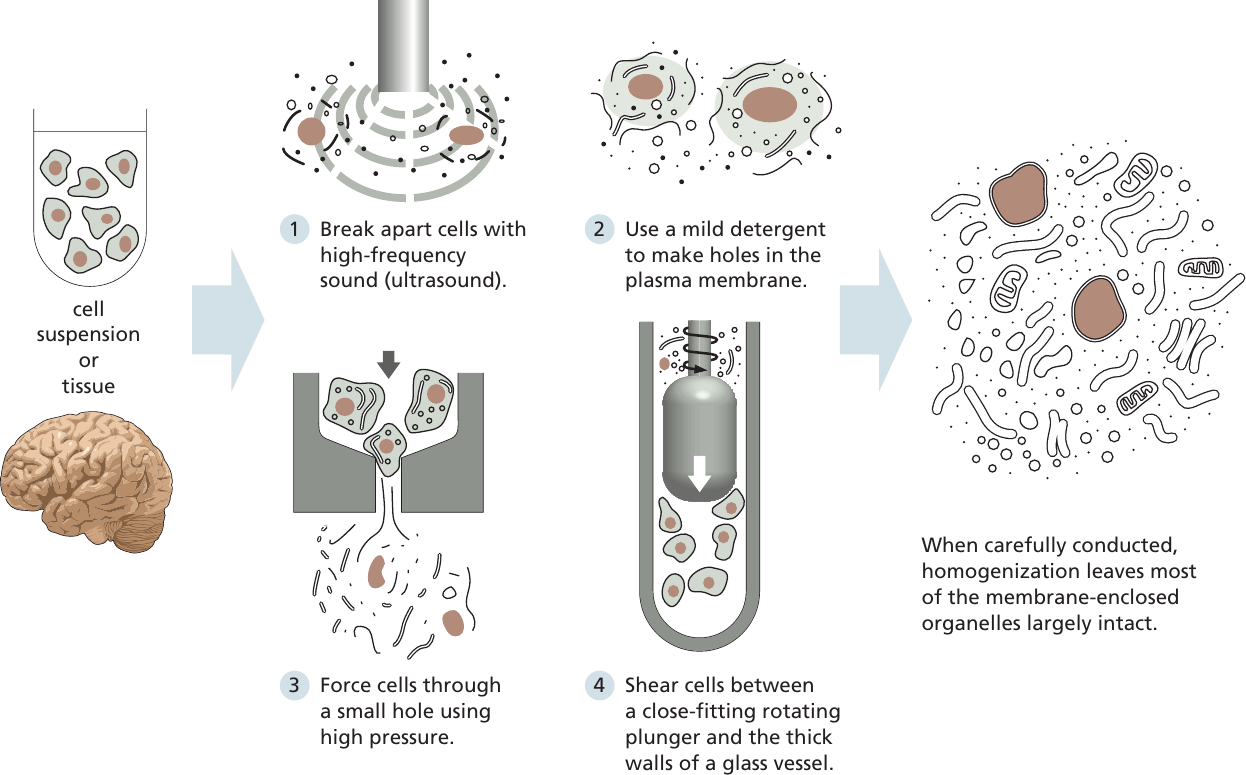
\includegraphics[scale=0.5]{images/break-cells.png}
		\caption{Omogenizzazione attraverso 4 diversi meccanismi, ognuno dei quali finalizzato a rompere le membrane plasmatiche. Fonte\cite{alberts2018essential}}
		\label{fig:break-cells}
	\end{figure}
	
	Segue poi una procedura di frazionamento iniziale, tipicamente per \textit{centrifugazione}, per separare l'omogenato in differenti parti. Per raggruppare poi le classi di molecole di interesse si possono usare tecniche di \textit{cromatografia} o \textit{elettroforesi}. Una forma efficiente di cromatografia è quella per \textit{affinità} nella quale vengono utilizzati degli anticorpi specifici per la proteina di interesse. Nel secondo metodo un insieme di proteine viene immerso in un gel e soggetto ad un campo elettrico: le proteine migreranno nel gel a differenti velocità, a seconda del loro peso molecolare e della loro carica. Proteine simili migreranno a velocità simili, pertanto potranno essere visualizzate bande o punti di aggregazione di proteine. \\
	
	\par Una volta separate le proteine di interesse è possibile studiarne la struttura. Per quanto riguarda la struttura primaria, la prima proteina sequenziata è stata l'\textit{insulina} nel 1955, attraverso una procedura chimica diretta. La proteina veniva prima scomposta da una determinata proteasi e successivamente ogni amminoacido, in ogni frammento, veniva determinato sperimentalmente. Un metodo molto più veloce è la \textit{spettrometria di massa}, almeno per organismi di cui sia stato completamente sequenziato il genoma. Questa tecnica determina l'esatta massa di ogni frammento in una proteina purificata, consentendo l'identificazione della proteina nei database di sequenze genomiche.
	
	\par Per eseguire la \textit{spettrometria di massa} la proteina viene "digerita" dall'enzima \textit{tripsina} e frammentata in peptidi o singoli amminoacidi. Questi vengono scaldati con un laser, il che li renderà carichi e li farà evaporare. Viene poi usato un potente campo elettrico per far volare gli ioni peptidici verso un misuratore: il tempo che impiegano per arrivare è legato alla loro massa e carica (più massa = più lenti, più carichi = più veloci). L'insieme delle precise masse dei frammenti serve come "impronta digitale" (\textit{peptide mass fingerprinting}, PMF) che verrà usata per identificare la proteina codificata dall'organismo (e i suoi geni corrispondenti) dai database il cui profilo (massa teorica) corrisponde a questa impronta peptidica.
	
	\subsubsection{Determinazione sperimentale delle strutture} \label{sec:determinazione-sperimentale}
	
	\par La determinazione sperimentale della struttura delle proteine ha vissuto dei progressi significativi col passare degli anni ed è di grande importanza per i metodi computazionali di PSP, consentendo ai metodi \textit{data-based} di affinare le loro predizioni.
	
	\begin{figure}[!htb]
		\centering
		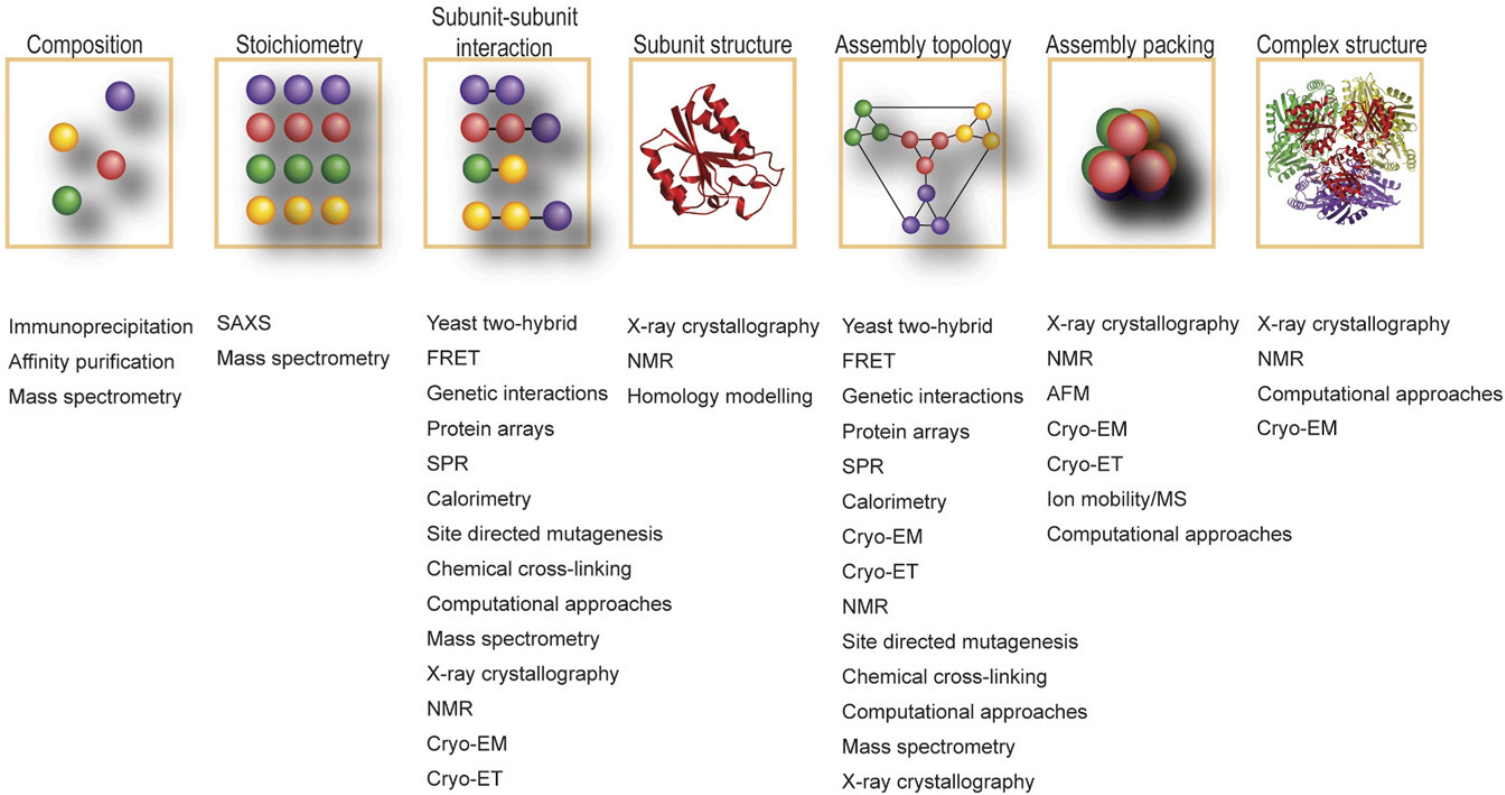
\includegraphics[scale=0.42]{images/metodi-sper2.png}
		\caption{Differenti livelli di informazione ottenuta lungo il percorso della determinazione della struttura di macromolecole. AFM: atomic force microscopy; Cryo-ET: cryo-electron tomography; EM: electron microscopy; FRET: fluorescence resonance energy-transfer; NMR: nuclear magnetic resonance; SAXS: small-angle X-ray scattering; SPR: surface plasmon resonance. Fonte\cite{sharon2011far}}
		\label{fig:metodi-sper2}
	\end{figure}
	
	I metodi per la determinazione sperimentale della struttura delle proteine possono essere divisi in due gruppi:
	\begin{itemize}
		\item metodi \textit{indiretti}, ovvero l'osservazione della proteina è possibile solo dopo sofisticate manipolazioni dei dati ottenuti:
		\begin{itemize}
			\item metodi per \textit{diffrazione}, che si basano sulla diffrazione o sulla dispersione di particelle subatomiche o onde elettromagnetiche da parte della proteina
			\item metodi per \textit{spettroscopia}, i quali si affidano all'eccitazione e susseguente rilassamento degli atomi della proteina in risposta alla radiazione elettromagnetica
		\end{itemize}
		\item metodi \textit{diretti}, in cui l'osservazione della proteina è diretta; al momento è possibile con la microscopia crioelettronica (Cryo-EM)
	\end{itemize}
	
	Vengono utilizzate principalmente 3 tecniche per generare informazioni strutturali sulle proteine a risoluzione atomica: \textit{X-ray crystallography, nuclear magnetic resonance (NMR) spectroscopy} ed \textit{electron microscopy}\footnote{La traduzione italiana sarebbe: cristallografia a raggi-X, spettroscopia a risonanza magnetica nucleare e microscopia elettronica.}. Una volta ottenute proteine pure, queste devono essere o cristallizzate (cristallografia a raggi X), o piazzate in speciali solventi (spettroscopia NMR) o congelate (microscopia elettronica). \\
	
	\par Il metodo di diffrazione più comune, e più anziano, è la \textit{cristallografia a raggi X}. Produce strutture tridimensionali con la più alta risoluzione ma presenta alcune gravi carenze, la più significativa è la necessità di cristallizzare la proteina studiata. La cristallizzazione è un processo lungo e difficile e produce anche strutture di proteine al di fuori del loro ambiente. Queste strutture sono prive di qualsiasi proprietà dinamica e (raramente) possono risultare deformate. Pertanto non tutte le parti di una proteina (ad es. le parti più mobili) possono essere viste con strutture a raggi-X e di conseguenza queste regioni possono essere ignorate o aperte a interpretazioni.
	
	\begin{figure}[!htb]
		\centering
		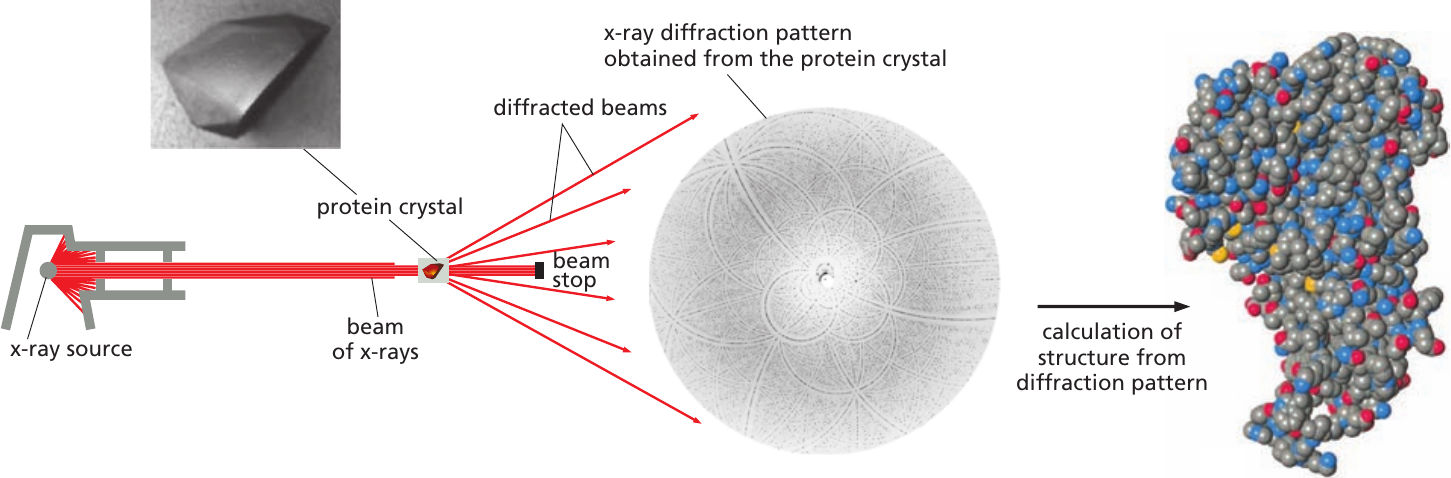
\includegraphics[scale=0.4]{images/cristallografia.png}
		\caption{Processo di determinazione della struttura dell'enzima RuBisCO tramite cristallografia a raggi-X. Fonte\cite{alberts2018essential}}
		\label{fig:cristallografia}
	\end{figure}
	
	\par I piccoli cristalli di proteine misurano meno di 1mm e sono esposti ad un'intensa esposizione ai raggi-X (i quali hanno una lunghezza d'onda pari a quella di un atomo, $1-2\angstrom$). I raggi X sono dispersi o diffratti dagli atomi proteici nel cristallo. Il modello di diffrazione che ne deriva appare tipicamente come decine di migliaia di minuscoli punti disposti in complessi schemi circolari. Questi modelli di diffrazione sono registrati su una fotocamera a raggi X digitale. La posizione dei punti di diffrazione (insieme ad altre informazioni), sono effettivamente sufficienti per compiere una computazione della mappa della densità elettronica di tutti gli atomi pesanti (carbonio, azoto, ossigeno, zolfo) nella proteina di diffrazione. Da questa mappa, i cristallografi determinano le coordinate x,y,z di tutti gli atomi usando la sequenza nota della proteina. Si noti che, nella cristallografia a raggi X, anche se il pattern di diffrazione deriva da milioni di proteine contenute nel cristallo, il risultato è una struttura per una singola proteina "media".
	
	\par La prima struttura determinata con questa tecnica risale al 1958; risolvere una struttura negli anni '70 richiedeva anche 6-7 anni mentre oggi è a volte possibile in soli 6-7 giorni. Il 90\% delle strutture oggi determinate deriva dalla cristallografia a raggi-X\supercite{baxevanis2020bioinformatics}. \\
	
	\par Altri metodi per diffrazione sono:  \textit{small-angle X-ray scattering }(SAXS), \textit{neutron scattering},  \textit{electron crystallography}. Il metodo SAXS produce strutture a risoluzione inferiore rispetto alla cristallografia a raggi X. Tuttavia, le strutture SAXS sono molto utili nell'impostare vincoli posizionali per complessi proteici di grandi dimensioni, grazie ai quali è possibile "modellare" strutture a raggi X ad alta risoluzione.
	
	\begin{figure}[!htb]
		\centering
		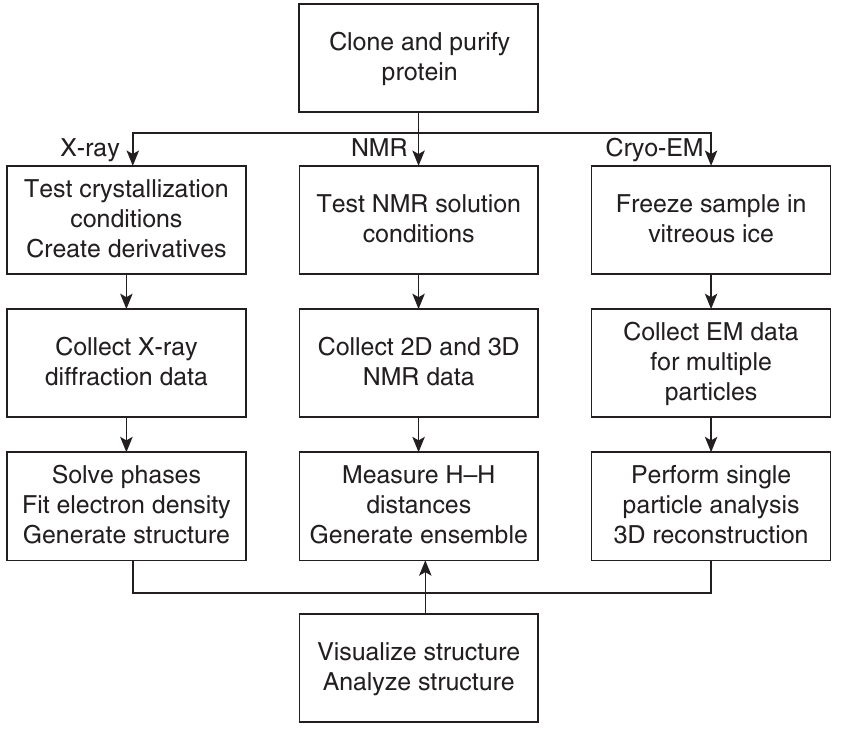
\includegraphics[scale=0.5]{images/metodi-sperimentali.png}
		\caption{Diagramma di flusso dei principali step usati la preparazione e soluzione sperimentale della struttura 3D delle proteine. Fonte\cite{baxevanis2020bioinformatics}}
		\label{fig:metodi-sper1}
	\end{figure}
	
	\par Il principale metodo spettroscopico utilizzato per la determinazione della struttura proteica è l'NMR. Questo metodo si basa sull'eccitazione dei nuclei atomici sotto un forte campo magnetico e sul loro successivo rilassamento. Viene misurato come i nuclei atomici (ad es. dell'idrogeno o dell'isotopo carbonio o azoto) assorbano la radiazioni; ciò permette di determinare quanto magnetismo nucleare è trasferito da un atomo all'altro. Questo approccio consente agli scienziati di trattare la proteina nel suo ambiente naturale (soluzione, membrana) e fornisce importanti informazioni sulla sua dinamica. L'NMR è un metodo più recente della cristallografia a raggi-X: la prima struttura determinata risale al 1983. Tuttavia questo metodo ha un limite superiore alla dimensioni di molecole studiabili (40kDa) e non può studiare proteine di membrana. L'EPR, un metodo simile, si basa sull'eccitazione e sul rilassamento degli elettroni attorno agli atomi della proteina e richiede la marcatura dei residui proteici con etichette paramagnetiche. \\
	
	\subsubsection{Cryo-EM}
	
	\par La microscopia crioelettronica (cryo-EM) è un metodo diretto: è possibile osservare direttamente macromolecole. È una versione avanzata di microscopio elettronico, il quale fu inventato negli anni '30. Questi microscopi usano raggi di elettroni piuttosto che di luce (la lunghezza d'onda degli elettroni è molto più corta di quella della luce). Durante la metà degli anni '70 è nata la cryo-EM: l'idea è stata quella di congelare i campioni per preservarne la struttura naturale e ridurre i danni causati dai raggi di elettroni.
	
	\begin{figure}[!htb]
		\minipage{0.5\textwidth}
		\centering
		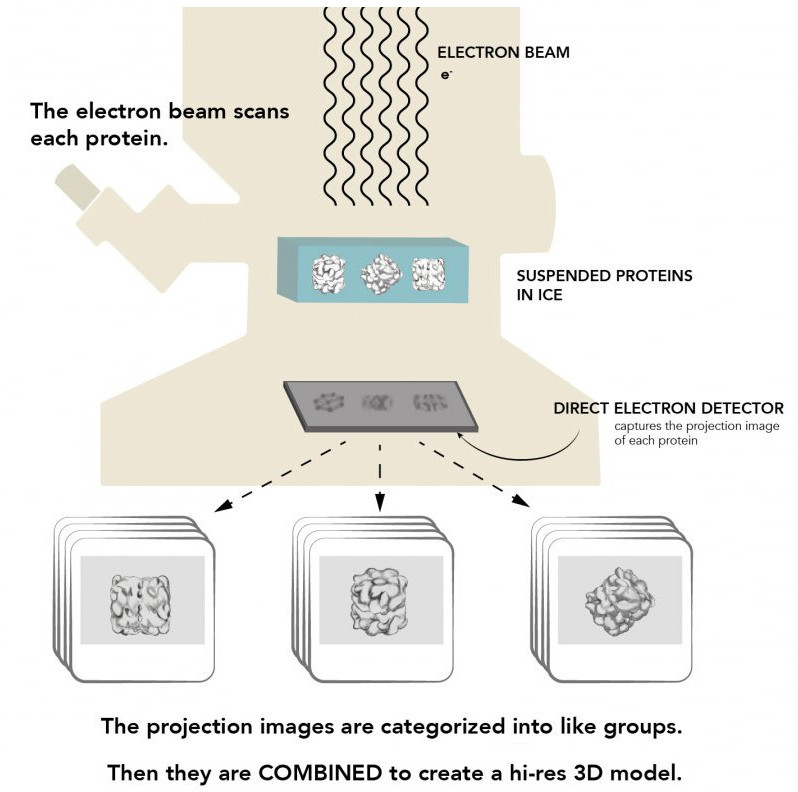
\includegraphics[scale=1.1]{images/cryo-em.jpg}
		\caption{Funzionamento schematico di un microscopio crio-elettronico. Fonte\cite{cryoEMbasics}}
		\label{fig:cryo-em-basics}
		\endminipage\hfill
		\minipage{0.5\textwidth}
		\centering
		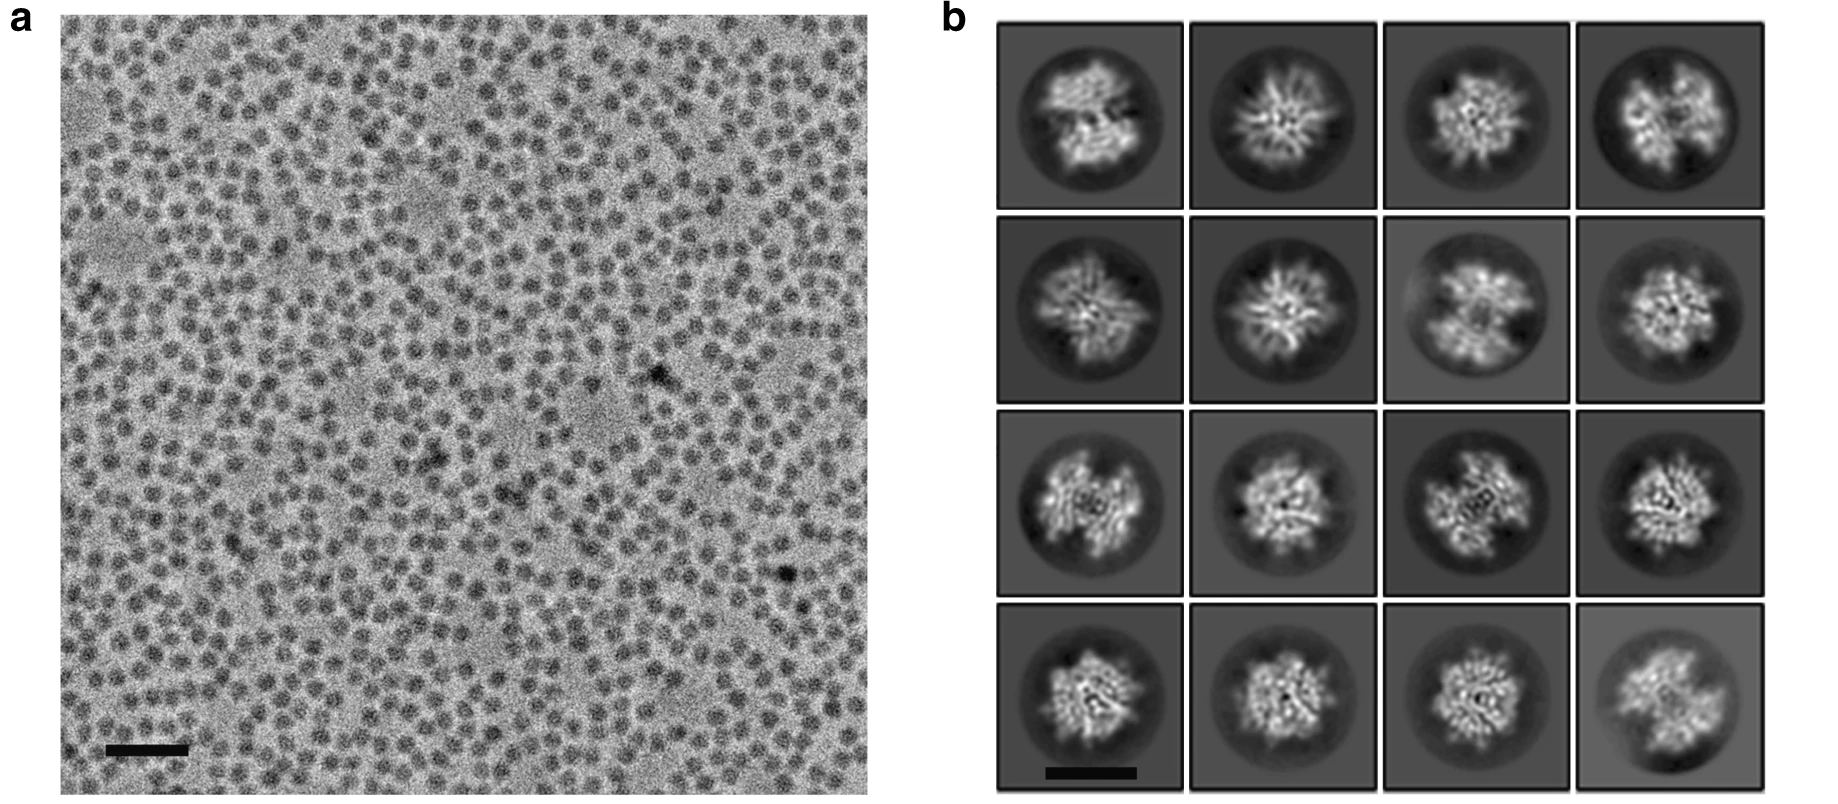
\includegraphics[scale=0.136]{images/cryo-em-classi.png}
		\caption{(A) Micrografia rappresentativa del campione di streptavidina ottenuta tramite cryo-EM. La barra di scala rappresenta 20nm (B) Classi medie 2D rappresentative delle immagini della proteina. La barra di scala rappresenta 5nm. Fonte \cite{fan2019single}}
		\label{fig:cryo-em-classi}
		\endminipage\hfill
	\end{figure}
	
	Nella cryo-EM una goccia di acqua contenente pure proteine è inserita in una piccola griglia per EM immersa in una vasca di etano liquido a -180°C. I campioni di proteine vengono congelati velocemente (creando ghiaccio vitreo): questo assicura che le circostanti molecole d'acqua non abbiano tempo per formare cristalli di ghiaccio (che deformerebbero la forma della proteina). I campioni sono esaminati (ancora ghiacciati) da un microscopio a trasmissione elettronica (TEM) e sottoposti quindi a forti raggi di elettroni. Un rilevatore di elettroni cattura le "immagini" proiettate delle molecole e, data l'automazione odierna di simili meccanismi, vengono effettuate migliaia di micrografie per catturare il maggior numero di dettagli possibile delle molecole. Ogni micrografia conterrà centinaia di migliaia di molecole singole, ognuna orientata casualmente. 
	\par Successivamente vi è lo step di image processing: le immagini proiettate vengono categorizzate in gruppi e allineate per poi essere sovrapposte in modo da calcolare un'immagine media per ogni gruppo. \\
	
	\par La preparazione è quindi molto più semplice rispetto alla cristallografia a raggi-X e le strutture somigliano maggiormente a quelle viste nel normale ambiente acquoso della cellula. La cryo-EM è limitata nelle dimensioni: c'è un limite inferiore che di anno in anno si abbassa (ad. es 39kDa nel 2019\supercite{fan2019single}). Non sono un problema invece grandi proteine (anche maggiori di 100kDa). Oggi la cryo-EM può generare immagini 3D a risoluzione quasi atomica di virus e complesse macromolecole, come i ribosomi. È possibile utilizzare la cryo-EM anche per le proteine di membrana. 
	
	\begin{figure}[!htb]
		\minipage{0.5\textwidth}
		\centering
		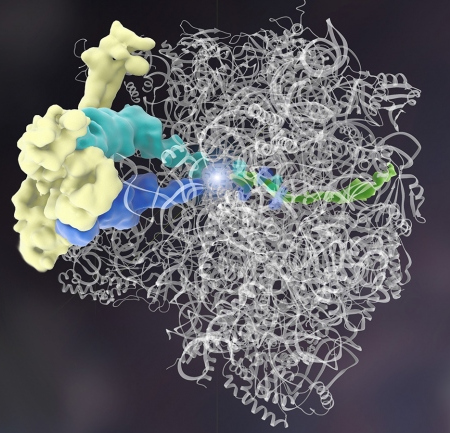
\includegraphics[scale=1.5]{images/cryo-ribosoma.jpg}
		\caption{Complesso di controllo qualità dei ribosomi, basato su dati di cryo-EM. Fonte: \cite{cryoRevolutionUCSF}}
		\label{fig:cryo-ribosoma}
		\endminipage\hfill
		\minipage{0.5\textwidth}
		\centering
		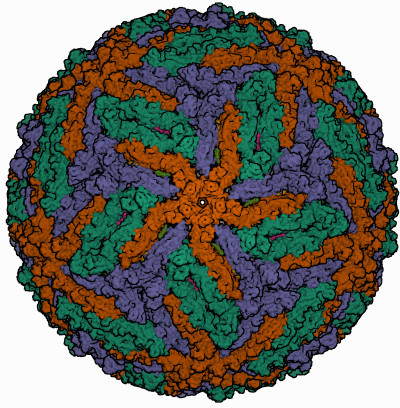
\includegraphics[scale=1.5]{images/cryo-zika.jpeg}
		\caption{La struttura del virus Zika ottenuta tramite cryo-EM. La macromolecola ha un peso di 190kDa ed è composta da 11.000 atomi. Risoluzione di 3.8\angstrom. Fonte \cite{cryoZika}}
		\label{fig:cryo-zika}
		\endminipage\hfill
	\end{figure}
	
	È solo da pochi anni che il metodo ha fatto un grande passo in avanti, grazie ad avanzamenti nel rivelatore e nei software di \textit{image processing}. Nel 2017 è stato assegnato il premio Nobel per la chimica per aver contribuito a sviluppare tale metodologia\footnote{A Richard Henderson, Jacques Dubochet e Joachim Frank, "for developing cryo-electron microscopy for the high-resolution structure determination of biomolecules in solution".}.
	Si sta considerando l'adozione della microscopia crioelettronica come di una rivoluzione nel campo della biologia strutturale\supercite{callaway2020revolutionary, bai2015cryo}. La crescita nel numero di strutture determinate è stata lenta inizialmente a causa della scarsa adozione del metodo, ma da quando si è vista la possibilità di produrre mappe dettagliate per macromolecole come i ribosomi la situazione è cambiata (vedi le figure \ref{fig:cryo-em-grafico} e \ref{fig:cryo-em-resolution}). Circa l'1\% delle strutture è stata determinata con questa tecnica ma i rapidi avanzamenti degli strumenti sia hardware che software potrebbero favorire la rivoluzione di cui si parla. 
	
	\begin{figure}[!htb]
		\minipage{0.58\textwidth}
		\centering
		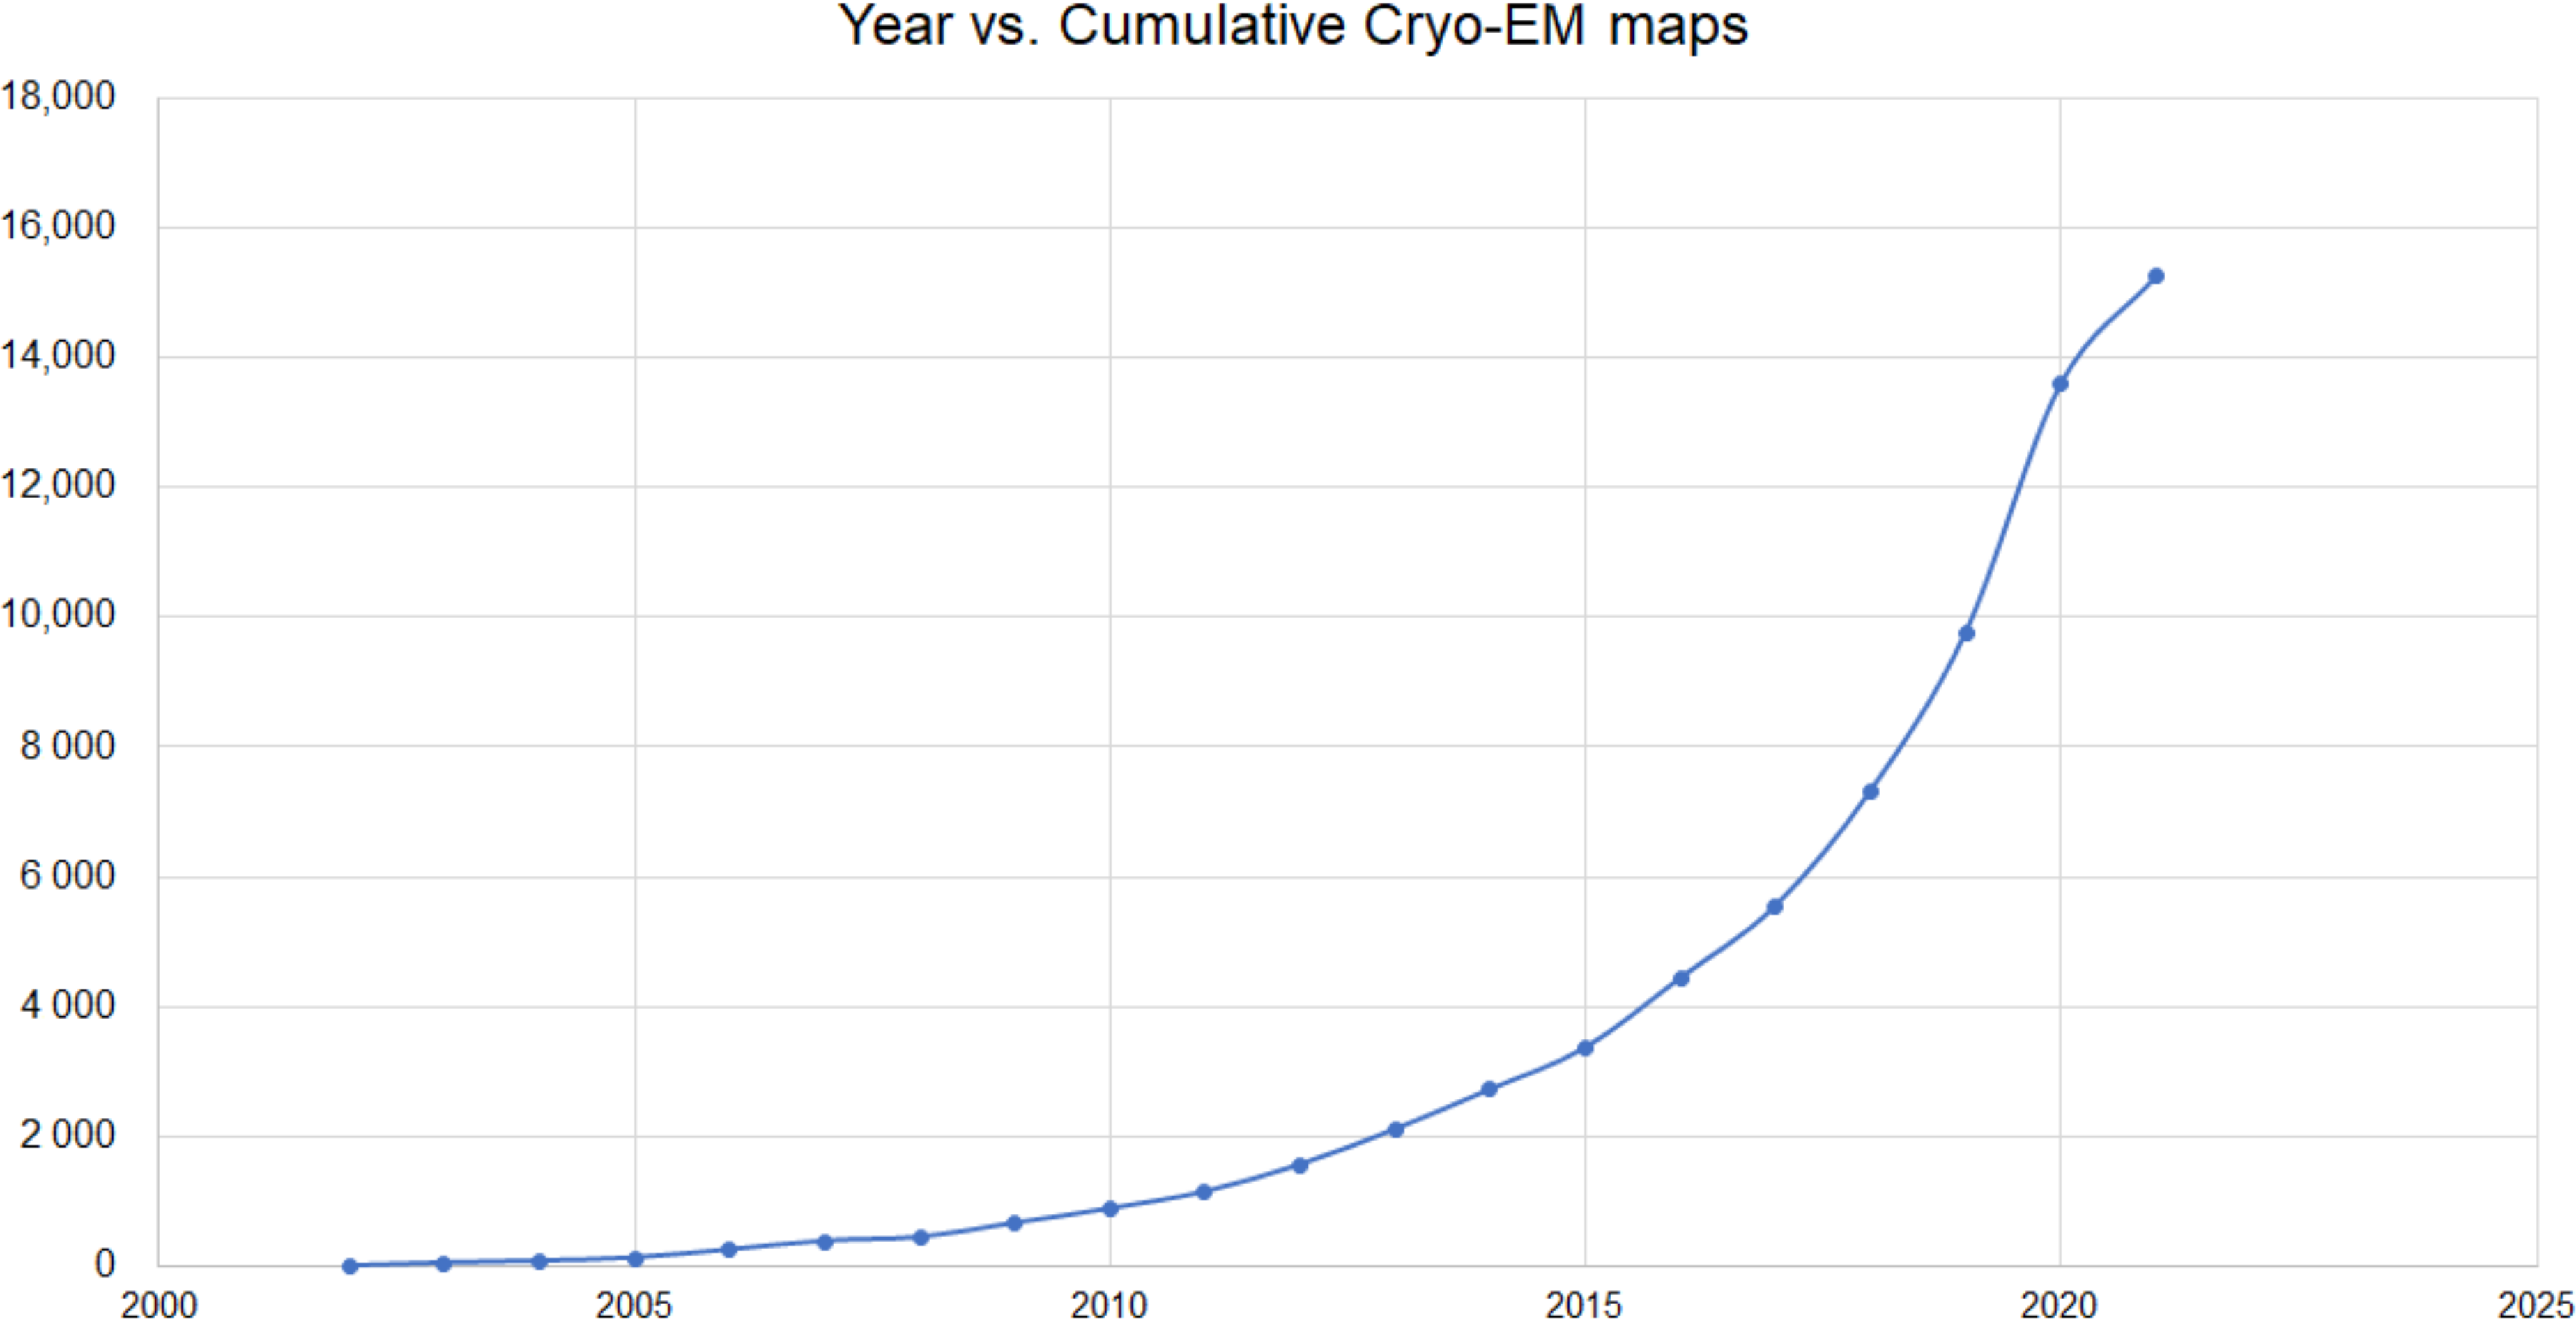
\includegraphics[scale=0.6]{images/cryo-em-grafico.png}
		\caption{Crescita delle mappe elettroniche rilasciate nell'EMDB. Fonte\cite{pakhrin2021deep}}
		\label{fig:cryo-em-grafico}
		\endminipage\hfill
		\minipage{0.4\textwidth}
		\centering
		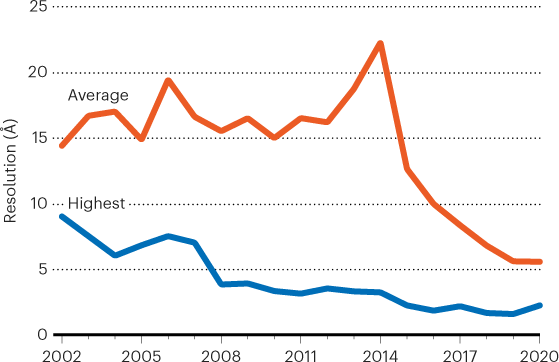
\includegraphics[scale=0.35]{images/cryo-em-resolution.png}
		\caption{Grafico della risoluzione di strutture risolte tramite cryo-EM. Fonte \cite{callaway2020revolutionary}}
		\label{fig:cryo-em-resolution}
		\endminipage\hfill
	\end{figure}
}

\section{Sfide al dogma di Anfinsen: IDP e fold switching} \label{sfide-dogma}
{
{

Il ripiegamento delle proteine in una cellula è un processo molto complesso che riguarda il trasporto di nuove proteine sintetizzate ad appropriati compartimenti cellulari attraverso targeting, misfolding, stati dispiegati temporanei, modifiche post-traduzione, controllo qualità, aggregazione in complessi, facilitazione dei chaperoni molecolari. Come già spiegato, l'aiuto dei chaperoni molecolari non sfida il dogma di Anfinsen, in quanto non influenza la struttura nativa della proteina.
	
\par La struttura di alcune proteine è difficile da determinare per una semplice ragione: un crescente numero di ricerche biochimiche ha rivelato che un numero significativo di proteine, o regioni di proteine, non hanno una distinta struttura 3D, non la hanno finché non interagiscono con la molecola target oppure cambiano struttura nativa. La loro flessibilità e struttura indefinita è importante per la loro funzione, che potrebbe richiedere legami con differenti target in tempi diversi. 

}

\subsubsection{Intrinsically disordered proteins}
Una proteina intrinsecamente disordinata (IDP) è una proteina, o una regione di essa, a cui manca una struttura terziaria fissa od ordinata. Le IDP sono comunemente riconosciute come regioni mancanti di densità elettronica in strutture di proteine determinate a cristallografia a raggi X. Molte IDP possono adottare una struttura tridimensionale stabile dopo essersi legate ad altre macromolecole, passando per transizioni disordine-ordine e perciò risultare strutturate per un certo periodo di tempo e non strutturate per altro. Ci sono però anche IDP che svolgono la loro funzione senza assumere mai una forma ordinata attraverso la loro esistenza.
Nonostante la loro mancanza di struttura stabile le IDP risultano essere una classe importante e grande di proteine.

\par Metodi bioinformatici suggeriscono che ?? la misura in le IDP sono prevalenti nel genoma di un organismo correla con la complessità dell'organismo in questione. Ciò implica che queste proteine giochino ruoli complessi. In accordo a studi bioinformatici su interi proteomi si stima che nei mammiferi circa il 25\% di tutte le proteine siano IDP e circa il 75\% di tutte le proteine di segnalazione (circa il 50\% di interi proteomi) contengano lunghe regioni disordinate\supercite{kessel_ben-tal_2018}.

\par Per tenere conto delle IDP in un modo che rifletta la loro prevalenza sono stati aperti diversi database liberamente disponibili ad esempio \href{http://www.disprot.org}{DisProt} e \href{http://MoBiDB.bio.unipd.it}{MoBiDB}.

\subsubsection{Fold switching proteins} \label{sec:fold-switching-proteins}
{
Alcune proteine hanno multiple strutture native: possono cambiare la loro forma, rimodellando anche le loro strutture secondarie, in base a fattori esterni. Ad esempio il complesso proteico KaiB cambia ripiegamento durante la giornata agendo da orologio per i cianobatteri. Si possono immaginare le proteine \textit{fold switching} come una sorta di transformer\footnote{La metafora è di Lauren Porter\supercite{porterYT}, autrice di \fullcite{porter2018extant}.} dove in un caso la proteina è come un robot che fa una cosa e in un altro caso, in risposta a cambiamenti ambientali, diventa un'automobile e fa qualcos'altro. Il cambio tra strutture alternative è guidato da interazioni della proteina con piccoli ligandi o altre proteine, da modificazioni chimiche (es. fosforilazione) o da cambiamenti nelle condizioni ambientali (temperatura, pH, potenziale di membrana). Ogni struttura alternativa può o corrispondere al minimo globale di energia libera della proteina in certe condizioni o essere cineticamente intrappolata in un minimo locale di energia libera\supercite{varela2019kinetic} circondato da alte barriere energetiche.

\par Le proteine \textit{fold switching} (FS) differiscono dalle IDP\supercite{porter2018extant}: 

\begin{itemize}
	\item le FS richiedono che entrambe le loro conformazioni siano determinate, le IDP sono regioni non determinate
	\item le IDP sono caratterizzate da sequenze amminoacidiche caratteristiche mentre le FS sono libere da questo vincolo
	\item le IDP non si ripiegano cooperativamente in isolamento mentre le FS si ripiegano sia cooperativamente che indipendentemente
\end{itemize}

Per queste ragioni si può affermare che le FS non sono IDP, piuttosto sono un sottoinsieme delle proteine globulari le cui strutture stabili cambiano drasticamente in risposta al loro ambiente. I vantaggi di una proteina FS sono legati alla sua bifunzionalità:
\begin{itemize}
	\item può affrontare velocemente richieste biologiche ovviando al bisogno di risorse cellulari aggiuntive per trascrivere e tradurre un'altra proteina. Un esempio è RfaH: funziona sia da fattore di trascrizione che di traduzione
	\item regolazione di inattività, può essere bloccata in uno stato di attività o inattività finché non viene innescato uno specifico segnale
\end{itemize}

È stato stimato che una percentuale tra lo 0.5 e il 4\% delle proteine nel PDB cambi ripiegamento\supercite{porter2018extant}.

}
\subsection{Considerazioni epistemologiche}
La scoperta delle IDP e delle proteine FS ha creato una spaccatura nel paradigma della struttura rigida delle proteine, secondo il quale la struttura deve essere fissa al fine di compiere la propria funzione biologica. È interessante ripercorrere velocemente la storia di questo paradigma attraverso un breve excursus storico per poterne mettere in luce le relazioni epistemologiche soggiacenti.

\par Nel 1894 Fischer ha proposto una metafora di \textit{chiave e serratura }per spiegare come fosse possibile un effetto chimico tra un enzima e un glucoside: \\
\say{\textit{Per usare una metafora, vorrei dire che l'enzima e il glucoside devono adattarsi l'uno all'altro come una serratura e una chiave per esercitare un effetto chimico l'uno sull'altro}\supercite{fischer1894einfluss}\supercite{dunker2001intrinsically}}

\par Nel 1936 Mirsky e Pauling hanno raccolto una quantità di informazioni sufficiente per concludere:\\
\say{\textit{attribuiamo le specifiche proprietà caratteristiche delle proteine native alle loro uniche e definite configurazioni. Consideriamo le proteine denaturate essere caratterizzate dall'assenza di un'unica definita configurazione\supercite{mirsky1936structure}}}.

Né Mirsky, né Pauling né Hsien Wu (probabilmente il primo a proporre il paradigma struttura unica-funzione) citarono il lavoro di Fischer ma la sua metafora avrebbe supportato pienamente le loro tesi. Perciò ancora prima dell'esperimento di Anfinsen e delle risoluzioni atomiche delle strutture, una specifica e ben ordinata forma tridimensionale era stata accettata come prerequisito essenziale per la funzione di una proteina.\supercite{dunker2001intrinsically}. Le prime strutture proteiche sono state determinate attraverso la cristallografia negli anni '50, dando ancora più credito all'ipotesi che una struttura fissa fosse necessaria per adempiere la funzione biologica. Queste pubblicazioni hanno contribuito a solidificare il dogma centrale della biologia molecolare. Nonostante questo già nel 1950 si parlava di molteplicità di strutture per una proteina, in particolare Karush\supercite{karush1950heterogeneity} sull'albumina del siero bovino, inferendo che le interazioni proteina-ligando stabilizzassero il membro più adatto da un insieme di strutture in equilibrio, chiamando questo fenomeno \textit{adattabilità configurazionale}. Successivamente si può ricordare il paradosso di Levinthal negli anni '60, per arrivare negli anni '70 al dogma di Anfinsen, il cui paradigma (sequenza amminoacidica $\dashrightarrow$ struttura tridimensionale $\dashrightarrow$ funzione) è messo in discussione da evidenze di mancanza di generalità. Tuttavia quel sistema di pensiero ha preso piede ed ha pervaso quasi tutti i lavori e teorie successive. Al tempo dell'esperimento di Anfinsen e delle prime risoluzioni atomiche della mioglobina e del lisozima il prerequisito di una forma tridimensionale fissa necessaria per la funzione della proteina era già accettato. La successiva valanga di migliaia di strutture determinate sperimentalmente ha contribuito ad affossare paradigmi di pensiero alternativi.

\par La scoperta di segmenti intrinsecamente disordinati è stata compiuta nel 1978, quando ancora erano disponibili le strutture di sole 20 proteine. Alcuni segmenti di proteine non fornivano alcuna densità elettronica distinguibile nonostante fossero essenziali per il funzionamento. Una  ragione comune è che gli atomi di quel segmento sono disordinati, ovvero la loro posizione cambia. Con l'avvento della spettroscopia NMR, sempre in quegli anni, si è arrivati a identificare intere proteine disordinate e dato che questo metodo è più preciso, la riscoperta di disordine nativo ha avuto un impatto significativo.

\par Fino al 2000\supercite{bracken2000disorder} queste idee non sono apparse nei libri di biochimica, nonostante in 50 anni fossero state pubblicate centinaia di paper sull'importanza della flessibilità e del disordine nelle strutture proteiche.

\par Può risultare interessante confrontare quanto accaduto con le analisi del microbiologo ed epistemologo Ludwik Fleck\supercite{fleck_1983}. Nel suo libro del 1935, \textit{Genesi e sviluppo di un fatto scientifico}, affronta il problema della conoscenza scientifica e analizza il caso dell'evoluzione del concetto della malattia sifilide, mostrando come questo si è modificato nel tempo. Senza entrare nel merito di quell'analisi, l'epistemologo ha provato a tracciare delle linee generali su come un fatto scientifico possa svilupparsi.

\par Analizzando le epoche di un concetto, Fleck si esprime affermando:\\
\say{\textit{Molte teorie, per esempio, hanno due epoche nella loro vita: esse attraversano prima un'epoca classica, in cui tutto si accorda in maniera impressionante, poi una seconda epoca, nel corso della quale si presentano solo delle eccezioni.}}

Non è difficile trovare le somiglianze con il caso della struttura unica per la funzione di una proteina. Inizialmente le eccezioni sono passate inosservate, tutto si accordava perfettamente all'idea di Fischer, Pauling e poi di Anfinsen. Le eccezioni, come quella di Karush, si presentavano ma il paradigma dominante non ne subiva effetti.

Secondo Fleck, per garantire la persistenza dei sistemi d'opinione quando si presentano eccezioni:\\
\say{\textit{una contraddizione al sistema appare impensabile. Ciò che non si accorda con il sistema: non viene notato, oppure viene taciuto anche se noto, oppure si fa in modo di spiegarlo, con laboriosi sforzi, come non contraddittorio rispetto al sistema: si notano, si descrivono o persino si inventano fatti che corrispondono alla concezione dominante, che cioè ne costituiscono per così dire la realizzazione}}\\

Uno dei concetti più importanti nell'opera di Fleck è il concetto di \textit{collettivo di pensiero} e \textit{stile di pensiero}:\\
\say{\textit{Se definiamo il termine collettivo di pensiero come "la comunità degli uomini che hanno fra loro un contatto intellettuale e che si scambiano idee influenzandosi reciprocamente, noi veniamo in possesso, con questo concetto, di ciò che rappresenta lo sviluppo storico di un ambito del pensiero, di un determinato patrimonio di conoscenza e di cultura e quindi, di un determinato stile di pensiero.}}

E secondo il microbiologo la condizione dell'individuo (scienziato) nei confronti dello stile di pensiero è di subordinazione inconsapevole:\\
\say{\textit{Anche se il collettivo consiste di individui, esso non è la loro semplice somma. L'individuo non ha mai - o quasi mai - la coscienza dello stile di pensiero collettivo, che quasi sempre esercita una costrizione incondizionata sul suo pensiero e che è semplicemente impensabile poter contraddire.}} \\

\say{\textit{Viene a anche a mettersi in luce che molte idee arrivano a manifestarsi prima che ne risaltino le basi razionali e, anzi, in modo completamente indipendente da queste ultime.}}
L'idea di Fischer (poi di Pauling) potrebbe avere influenzato il collettivo di pensiero al punto tale che la determinazione delle prime strutture a risoluzione atomica non potesse che dare come risposta una conferma di quelle idee. Esperimento ed esperienza non vivono entrambe nel campo dell'oggettività:\\
\say{\textit{se l'esperimento può essere interpretato come una pura e semplice domanda e risposta, l'esperienza deve essere invece intesa già come una condizione complessa, frutto di un processo di educazione che si fonda sull'interazione fra chi conosce, ciò che è conosciuto e ciò che deve essere conosciuto.}} 

La mancata consapevolezza di far parte di un collettivo di pensiero può purtroppo causare l'illusione che esista un nesso logico fra prove e concezioni, ma Fleck ammonisce: \\
\say{\textit{le prove si adattano alle concezioni altrettanto spesso quanto le concezioni si conformano alle prove}}

Secondo Fleck la conoscenza è sempre un processo sociale:\\
\say{"\textit{questo libro è più voluminoso}" \textit{è incompleta. Sarebbe corretta se si aggiungesse }"\textit{di quel libro}"\textit{; [..] la frase }«\textit{qualcuno conosce qualcosa}» \textit{richiede un'aggiunta, ad es.} "\textit{sulla base di un determinato patrimonio di conoscenza}" \textit{o meglio }"\textit{come membro di un determinato ambiente culturale}" \textit{o ancora }"\textit{in un determinato collettivo di pensiero}"}

Mettendo insieme le diverse constatazioni riportate si può fare un'analisi, senza alcuna presunzione di correttezza e come semplice esercizio, del dogma di Anfinsen. Secondo Fleck una formulazione corretta sulle sue scoperte potrebbe essere: "Anfinsen propose, in conformità con le opinioni del suo tempo sul ripiegamento, denaturazione e rinaturazione delle proteine, di vedere nella sequenza amminoacidica la base necessaria e sufficiente per la determinazione della sua struttura tridimensionale nativa. Propone inoltre, sempre sulla base del collettivo di pensiero in cui era immerso, di considerare la struttura nativa di una proteina come quella struttura unica, stabile e cineticamente accessibile avente minima energia libera". Da questo esercizio si può osservare, essendo noi immersi in un collettivo di pensiero differente, che lo stile di pensiero di Anfinsen era probabilmente ancorato alle idee di Pauling secondo il quale la conformazione stabile delle proteine era una e una soltanto.
}

\section{Il problema del Protein Folding} \label{sec:problema-protein-folding}
{
Il problema del protein folding è la questione di \textit{come} una sequenza amminoacidica determini la struttura atomica tridimensionale. Il processo del ripiegamento proteico non è così semplice, la maggior parte delle proteine probabilmente passa attraverso strutture intermedie sulla via per raggiungere la struttura nativa, e il semplice osservare la struttura finale non rivela i passaggi del ripiegamento richiesti per raggiungere quella forma. Il problema del protein folding consiste di 3 puzzle strettamente correlati\supercite{dill2008protein}:
\begin{itemize}
	\item \textit{folding code}: la questione termodinamica di quale bilancio delle forze interatomiche determini la struttura della proteina a partire da una data sequenza amminoacidica
	
	\item \textit{folding process}: la questione cinetica di quali percorsi alcune proteine usino per ripiegarsi così velocemente
	
	\item\textit{protein structure prediction}: si può predire la struttura nativa di una proteina dalla sua sequenza amminoacidica? In altre parole il problema computazionale di come predire la struttura nativa di una proteina dalla sua sequenza amminoacidica
	
\end{itemize}	

Il problema del protein folding, come si può immaginare, è considerato uno dei problemi più impegnativi degli ultimi 50 anni in biochimica, ed è stato fatto riferimento alla predizione della struttura delle proteine come al \textit{santo Graal} della biochimica computazionale\supercite{abbass2020enhancing}. Sfortunatamente esso è stato anche rivendicato come uno dei problemi di ottimizzazione più complicati che gli informatici abbiano mai affrontato\supercite{abbass2020enhancing}.

\subsubsection{Paradosso di Levinthal}

 Un aspetto importante del problema è sottolineato dal \textit{paradosso di Levinthal}. Nel 1968 Cyrus Levinthal\supercite{levinthal1969fold} si rese conto che, a causa dell'elevato numero di gradi di libertà di un polipeptide non ripiegato, tale molecola presenterebbe un numero astronomico di possibili conformazioni finali. Se la proteina raggiungesse la sua conformazione finale passando via via attraverso tutte queste configurazioni, sarebbe necessario un tempo ben superiore all'età attualmente stimata dell'universo per raggiungere la configurazione corretta, anche se ogni passaggio richiedesse pochi \textit{picosecondi}\footnote{Levinthal stima $10^{300}$ possibili conformazioni teoriche per una proteina di 2000 atomi\supercite{levinthal1969fold}.}.
 
 \par Prendendo ad esempio un polipeptide di 100 residui si avranno 99 legami peptidici e di conseguenza 198 differenti angoli di legame $\phi$ e $\psi$. Assumendo che ognuno di questi angoli possa esistere in ognuna delle 3 configurazioni stabili la proteina potrebbe assumere fino a $3^{198}$ configurazioni (includendo ogni possibile ridondanza di ripiegamento).
 
\par In natura però molte piccole proteine si ripiegano spontaneamente in un tempo dell'ordine dei millisecondi o addirittura dei microsecondi. Il tempo di generazione di E. coli può essere di circa venti minuti: ciò significa che tutte le proteine essenziali per tale organismo (e presumibilmente di tutti gli altri) possono essere prodotte da zero in un tempo decisamente ristretto, al massimo nell'ordine dei minuti.

\par Il processo di ripiegamento non è quindi una ricerca all'interno dell'enorme spazio degli stati configurazionali possibili. La differenza enorme che esiste tra il tempo del ripiegamento prevedibile in teoria e quello osservato in realtà è appunto chiamato paradosso di Levinthal. \\

\par Come accennato nella sezione \ref{sec:assisted-folding}, la malattia di Alzheimer, la fibrosi cistica e altre malattie neurodegenerative sono associate al mal ripiegamento delle proteine. La conoscenza dei fattori di mal ripiegamento e la comprensione del processo di ripiegamento proteico potrebbero aiutare nello sviluppo di cure per queste malattie. Per queste ragioni è importante anche rispondere alle altre domande del problema e non fermarsi alla predizione della struttura finale, nonostante questa conoscenza fornisca un grande vantaggio per lo sviluppo di nuovi farmaci e il design di nuove proteine.
}
\clearpage